\documentclass[11pt,a4paper]{article}
\usepackage[utf8]{inputenc}
\usepackage{amsmath,amssymb,amsthm}
\usepackage{mathrsfs}
\usepackage{hyperref}
\usepackage{microtype}
\usepackage{longtable}
\usepackage{booktabs}
\usepackage{array}
\usepackage{adjustbox}
\usepackage{ragged2e}
\usepackage[margin=1in]{geometry}
\usepackage{enumitem}
\usepackage{tikz}
\usetikzlibrary{arrows.meta,positioning,shapes.geometric,fit,backgrounds,calc}
\usepackage{float}
\usepackage{xcolor}
\usepackage{listings}

% Listing styles
\lstdefinestyle{leanproved}{
  language={},
  basicstyle=\ttfamily\footnotesize,
  breaklines=true,
  breakatwhitespace=false,
  columns=fullflexible,
  keepspaces=true,
  frame=single,
  backgroundcolor=\color{green!6},
  rulecolor=\color{green!40!black},
  xleftmargin=0.5em, framexleftmargin=0.5em,
}
\lstdefinestyle{leanaxiom}{
  language={},
  basicstyle=\ttfamily\footnotesize,
  breaklines=true,
  breakatwhitespace=false,
  columns=fullflexible,
  keepspaces=true,
  frame=single,
  backgroundcolor=\color{orange!8},
  rulecolor=\color{orange!70!black},
  xleftmargin=0.5em, framexleftmargin=0.5em,
}
\lstdefinestyle{leansorry}{
  language={},
  basicstyle=\ttfamily\footnotesize,
  breaklines=true,
  breakatwhitespace=false,
  columns=fullflexible,
  keepspaces=true,
  frame=single,
  backgroundcolor=\color{red!6},
  rulecolor=\color{red!50!black},
  xleftmargin=0.5em, framexleftmargin=0.5em,
}
\lstset{
  style=leanproved,
  literate=
    {⁻¹}{{$^{-1}$}}2
    {∀ᵐ}{{$\forall^{\mathrm{m}}$}}2
    {¬}{{$\neg$}}1
    {¹}{{$^1$}}1
    {Λ}{{$\Lambda$}}1
    {ε}{{$\varepsilon$}}1
    {ζ}{{$\zeta$}}1
    {η}{{$\eta$}}1
    {μ}{{$\mu$}}1
    {ν}{{$\nu$}}1
    {σ}{{$\sigma$}}1
    {φ}{{$\phi$}}1
    {χ}{{$\chi$}}1
    {ψ}{{$\psi$}}1
    {ᵐ}{{$^{\mathrm{m}}$}}1
    {ᶜ}{{$^{\mathrm{c}}$}}1
    {‖}{{$\Vert$}}1
    {⁻}{{$^{-}$}}1
    {↑}{{$\uparrow$}}1
    {∀}{{$\forall$}}1
    {∂}{{$\partial$}}1
    {∈}{{$\in$}}1
    {∉}{{$\notin$}}1
    {∑}{{$\sum$}}1
    {∩}{{$\cap$}}1
    {∫}{{$\int$}}1
    {≠}{{$\neq$}}1
    {≤}{{$\le$}}1
    {⊆}{{$\subseteq$}}1
    {⟨}{{$\langle$}}1
    {⟩}{{$\rangle$}}1
}
\urlstyle{tt}
\setlength{\emergencystretch}{3em}
\setlength{\LTleft}{0pt}
\setlength{\LTright}{0pt}

\newtheorem{theorem}{Theorem}[section]
\newtheorem{lemma}[theorem]{Lemma}
\newtheorem{proposition}[theorem]{Proposition}
\newtheorem{corollary}[theorem]{Corollary}
\newtheorem{definition}[theorem]{Definition}
\newtheorem{remark}[theorem]{Remark}

\newcommand{\Schwartz}{\mathscr{S}}
\newcommand{\Sprime}{\mathscr{S}'}
\newcommand{\ZDS}{\mathrm{ZDS}}
\newcommand{\OS}{\mathrm{OS}}
\newcommand{\BHW}{\mathrm{BHW}}
\newcommand{\CLM}{\mathrm{CLM}}
\newcommand{\sorry}{\texttt{sorry}}
\newcolumntype{L}[1]{>{\RaggedRight\arraybackslash}p{#1}}
\newcommand{\leanfile}[1]{\begingroup\Urlmuskip=0mu plus 1mu\relax\nolinkurl{#1}\endgroup}
\newcommand{\leanname}[1]{\begingroup\Urlmuskip=0mu plus 1mu\relax\nolinkurl{#1}\endgroup}

\title{Lean 4 Formalization of the Osterwalder--Schrader Reconstruction Theorem:\\
Comprehensive Proof Notes with OS Paper Comparison}
\author{OSReconstruction Project}
\date{March 23, 2026}

\begin{document}
\sloppy
\maketitle

\begin{abstract}
We present a comprehensive account of the Lean~4 formalization of the
Osterwalder--Schrader reconstruction theorem, mapping the formal proof to the
original OS~I~\cite{OS1} and OS~II~\cite{OS2} papers. We cover the complete
$E \to R$ and $R \to E$ directions, the GNS Hilbert space construction,
the Bargmann--Hall--Wightman theorem, boundary value transfers, and all
supporting infrastructure. Every Lean definition, theorem, axiom, and
\sorry{} obligation is presented with its full formal signature and
mathematical explanation.

\medskip\noindent
\textbf{Status note.} The critical-path sections of this note have been updated
to the current production route as of 2026-03-23. In particular, the active
$E \to R$ frontier now follows the corrected OS~II semigroup/VI.1 route through
\leanfile{OSToWightmanK2VI1.lean}; older fixed-probe two-point kernel detours
are no longer on the production critical path.

\medskip\noindent
\textbf{Status convention used in this note.}
Whenever a main theorem or package is marked as ``proved,'' the note now tries to
distinguish four cases:
\begin{itemize}
\item \textbf{sorry-free} = the declaration is present in Lean and its dependency
  audit does \emph{not} show \texttt{sorryAx} or project axioms;
\item \textbf{sorry-dependent} = the declaration exists in Lean, but
  \texttt{\#print axioms} shows \texttt{sorryAx} and/or a project axiom in its trust
  boundary;
\item \textbf{axiom-dependent but sorry-free} = the declaration has no
  \texttt{sorryAx} in its trust boundary, but still depends on an explicit
  project axiom such as \leanname{schwartz\_nuclear\_extension};
\item \textbf{open} = the declaration still contains an explicit \sorry{};
\item \textbf{axiomatic} = the declaration is introduced as an axiom.
\end{itemize}

\noindent
When a file-level support layer rather than a single theorem is being described,
the note says so explicitly instead of silently treating file completion as a
theorem-status claim.

\medskip\noindent
Whenever possible, the note also distinguishes three ways a declaration can look
``finished'' in source code: it may be genuinely sorry-free and axiom-free; it
may be sorry-free but still inherit a project axiom; or it may exist in Lean
while still inheriting \texttt{sorryAx} from unresolved support work.

\medskip\noindent
\textbf{Listing color code:}
\colorbox{green!6}{\strut Green} = sorry-free declaration shown verbatim.
\colorbox{orange!8}{\strut Orange} = Lean axiom.
\colorbox{red!6}{\strut Red} = explicit \sorry{} / open obligation.

\medskip\noindent
\textbf{Important reading rule for code excerpts.}
Some Lean snippets below retain source-style comments such as ``(PROVED)'' because
they are documenting what the source file says locally. Those comments should not
be read by themselves as dependency audits. Whenever the note discusses a main
theorem or route-defining declaration, the dependency-aware status is given in the
surrounding prose, charts, or tables.
\end{abstract}

\tableofcontents
\newpage

%% ===================================================================
\part{Overview and Dependency Structure}
%% ===================================================================

\section{Introduction}

The Osterwalder--Schrader reconstruction theorem establishes a bijection
between:
\begin{itemize}
\item \textbf{Euclidean quantum field theories}, specified by Schwinger
  functions $\{\mathfrak{S}_n\}$ satisfying axioms E0--E4, and
\item \textbf{Relativistic quantum field theories}, specified by Wightman
  distributions $\{\mathfrak{W}_n\}$ satisfying axioms R0--R5.
\end{itemize}

The correspondence consists of two directions:
\begin{description}
\item[$E \to R$:] Given Schwinger functions, construct Wightman distributions
  via a Hilbert space (GNS construction), contraction semigroup, and analytic
  continuation.
\item[$R \to E$:] Given Wightman distributions, construct Schwinger functions
  by evaluating the analytic continuation (Bargmann--Hall--Wightman theorem)
  at Euclidean points via Wick rotation.
\end{description}

\subsection{Current Status Note (2026-03-23)}

The repository has recently undergone a substantial course correction on the
$E \to R$ side.

\begin{itemize}
\item The production route now follows the OS papers strictly: semigroup/Hilbert
  space first, then the OS~II Section~VI.1 regularization and boundary-value
  identification, and only afterwards the general several-complex-variables
  continuation and boundary-value transfer chain.
\item The older specialized two-point kernel / \texttt{differenceLift} detours
  have been removed from the active production path and moved out of the live
  route. They should be regarded as deprecated historical explorations, not as
  current blockers.
\item The honest Euclidean surface in this project is the zero-diagonal Schwartz
  space. No current production theorem on the $E \to R$ route is allowed to
  replace that by a full-Schwartz Euclidean surrogate merely for convenience.
\item On the $R \to E$ side, the repo still contains historical route issues,
  especially around reduced-coordinate BHW infrastructure. Those are currently
  flagged but not the implementation focus.
\end{itemize}

\subsection{Current Production Blockers}

The current blocker map is best understood at the file/theorem level.

\paragraph{E-to-R active route.}
\begin{enumerate}
\item \leanfile{OSToWightmanSemigroup.lean} is the proved one-variable OS
  semigroup/Laplace layer.
\item \leanfile{OSToWightmanK2BaseStep.lean} is the proved support layer for the
  honest $k=2$ route: canonical probe witness, Bochner measure, positive-time
  shell identities, Laplace--Fourier reduction, and auxiliary support/control
  lemmas.
\item \leanfile{OSToWightmanK2VI1.lean} is the live OS~II Section~VI.1 frontier.
  The two active open theorems there are:
  \begin{itemize}
  \item \leanname{translatedProductShell_boundary_tendsto_schwingerDifferencePositive_of_negativeApproxIdentity_local}
  \item \leanname{exists_k2_timeParametric_distributional_assembly}
  \end{itemize}
  The first is the sequence-level VI.1 boundary-limit theorem; the second is the
  final $k=2$ existential assembly theorem above that limit.
\item \leanfile{OSToWightman.lean} contains the next two live general-$k$
  blockers:
  \begin{itemize}
  \item \leanname{exists_acrOne_productTensor_witness}
  \item \leanname{acrOne_productTensor_witness_extends_zeroDiagonal}
  \end{itemize}
  These are the OS-II several-complex-variables / Osgood / product-tensor
  continuation steps above the solved $k=2$ base.
\item \leanfile{OSToWightmanBoundaryValues.lean} is the downstream boundary-value
  transfer lane. Its live front is \leanname{boundary_values_tempered}, followed
  by the remaining transfer theorems in that file.
\end{enumerate}

\paragraph{R-to-E flagged route.}
Implementation work is not currently focused here, but the live front remains in
\leanfile{SchwingerTemperedness.lean}, \leanfile{SchwingerAxioms.lean},
\leanfile{ForwardTubeLorentz.lean}, \leanfile{BHWTranslation.lean}, and the
deferred reduced-BHW bridge axiom in \leanfile{BHWReducedExtension.lean}.
There is also an upstream analytic-geometry dependency in
\leanfile{ComplexLieGroups/Connectedness/BHWPermutation/PermutationFlowBlocker.lean}.

\subsection{Repository Structure}

The Lean~4 formalization lives in four modules:
\begin{itemize}
\item \texttt{Wightman/} --- Wightman axioms, GNS construction, reconstruction
\item \texttt{SCV/} --- Several complex variables (identity theorems, tube domains,
  Fourier--Laplace, Bochner tube theorem)
\item \texttt{ComplexLieGroups/} --- Complex Lorentz group, connectedness,
  BHW permutation flow
\item \texttt{vNA/} --- Von Neumann algebras (spectral theory, modular theory,
  Stone's theorem)
\end{itemize}

\medskip\noindent
\textbf{Deprecated route material.}
The repository also contains
\leanfile{Wightman/Reconstruction/WickRotation/deprecated/}. Those files are
not on the live production route. They archive earlier route experiments,
especially the removed two-point-kernel / \texttt{differenceLift} detours from
the $E \to R$ direction, and should be read as historical context rather than as
current proof obligations.

\section{Current Critical Paths}

\subsection{E-to-R Critical Path}

The active production $E \to R$ path is now the strict OS-route chain shown
below.

\begin{center}
\begin{adjustbox}{max width=\textwidth,center}
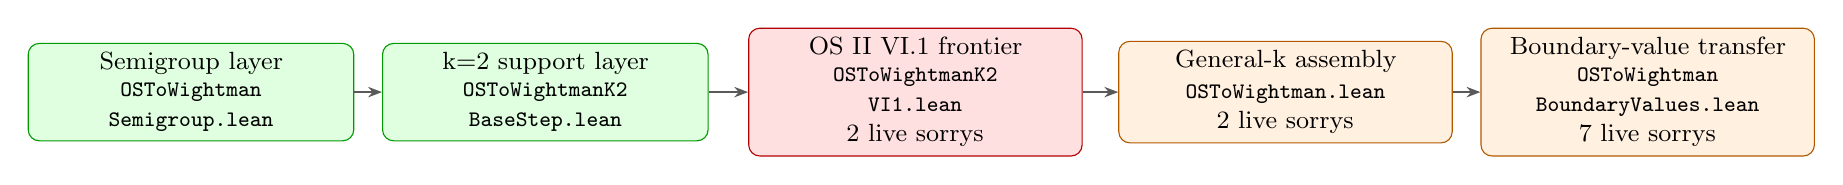
\begin{tikzpicture}[
  proved/.style={rectangle, rounded corners, draw=green!60!black, fill=green!12,
    text width=3.9cm, minimum height=1.1cm, align=center, font=\small},
  frontier/.style={rectangle, rounded corners, draw=red!70!black, fill=red!12,
    text width=4.0cm, minimum height=1.2cm, align=center, font=\small},
  pending/.style={rectangle, rounded corners, draw=orange!70!black, fill=orange!12,
    text width=4.0cm, minimum height=1.1cm, align=center, font=\small},
  arr/.style={-{Stealth[length=5pt]}, thick, gray!70!black},
]
\node[proved] (s) at (0,0)
  {Semigroup layer\\{\footnotesize\texttt{OSToWightman}\\\texttt{Semigroup.lean}}};
\node[proved] (k2b) at (4.5,0)
  {k=2 support layer\\{\footnotesize\texttt{OSToWightmanK2}\\\texttt{BaseStep.lean}}};
\node[frontier] (vi1) at (9.2,0)
  {OS II VI.1 frontier\\{\footnotesize\texttt{OSToWightmanK2}\\\texttt{VI1.lean}}\\2 live sorrys};
\node[pending] (gen) at (13.9,0)
  {General-k assembly\\{\footnotesize\texttt{OSToWightman.lean}}\\2 live sorrys};
\node[pending] (bv) at (18.5,0)
  {Boundary-value transfer\\{\footnotesize\texttt{OSToWightman}\\\texttt{BoundaryValues.lean}}\\7 live sorrys};
\draw[arr] (s) -- (k2b);
\draw[arr] (k2b) -- (vi1);
\draw[arr] (vi1) -- (gen);
\draw[arr] (gen) -- (bv);
\end{tikzpicture}
\end{adjustbox}

\medskip
\textbf{Flow chart:} current strict OS-route $E \to R$ critical path.
\end{center}

{\scriptsize
\begin{longtable}{@{}L{0.23\textwidth}L{0.17\textwidth}L{0.54\textwidth}@{}}
\toprule
\textbf{File} & \textbf{Status} & \textbf{Role on the critical path} \\
\midrule
\endhead
\leanfile{OSToWightmanSemigroup.lean} & mixed proved layer &
OS semigroup, spatial-translation, spectral/Laplace, and one-variable
holomorphic infrastructure. \\
\leanfile{OSToWightmanK2BaseStep.lean} & compile-closed support layer &
All proved support machinery for the honest $k=2$ route:
canonical probe witness, Bochner package, positive-time shell identities,
Laplace--Fourier bridges, and support control. \\
\leanfile{OSToWightmanK2VI1.lean} & 2 open theorems &
Current live frontier. This file isolates the remaining OS~II VI.1
regularization/boundary-identification step and the final $k=2$ existential
assembly theorem. \\
\leanfile{OSToWightman.lean} & 2 private open theorems &
General-$k$ Osgood / product-tensor witness layer above the solved $k=2$ base. \\
\parbox[t]{0.23\textwidth}{\ttfamily OStoWightman\\BoundaryValues.lean} & 7 open theorems &
Tempered boundary-value packaging and the downstream transfer theorems needed to
finish the final $E \to R$ assembly. \\
\bottomrule
\end{longtable}
}

\paragraph{Important correction.}
Any diagram or discussion that routes the active $E \to R$ proof through a
specialized fixed-probe two-point kernel theorem is now obsolete. The current
route uses the sequence-level OS~II VI.1 regularization theorem in
\leanfile{OSToWightmanK2VI1.lean}; the fixed-probe surface was removed because
it was stronger than the paper route and risked targeting the wrong theorem.

\medskip\noindent
These file-level labels summarize route position, not theorem trust boundaries.
Below, whenever a specific declaration is named, the note states separately
whether it is sorry-free, axiom-dependent but sorry-free, sorry-dependent, or
open.

\subsection{R-to-E Critical Path}

The current $R \to E$ story should be read more cautiously. It is not the active
implementation focus, and its route has \emph{not} yet received the same strict
course correction as $E \to R$. The live blockers remain distributed across:
\begin{itemize}
\item \leanfile{SchwingerTemperedness.lean} --- zero-diagonal continuity front
\item \leanfile{SchwingerAxioms.lean} --- Euclidean reality/reflection/cluster lane
\item \leanfile{ForwardTubeLorentz.lean} --- analytic-geometry upstream blockers
\item \leanfile{BHWTranslation.lean} --- residual translation-invariance blocker
\item \leanfile{BHWReducedExtension.lean} --- deferred reduced-BHW bridge axiom
\item \leanfile{ComplexLieGroups/Connectedness/BHWPermutation/PermutationFlowBlocker.lean}
  --- permutation-flow connectedness blockers upstream of the BHW lane
\end{itemize}

So any older diagram that presents the $R \to E$ side as a settled linear chain
should now be read as schematic rather than as an accurate current blocker map.

\begin{center}
\begin{adjustbox}{max width=\textwidth,center}
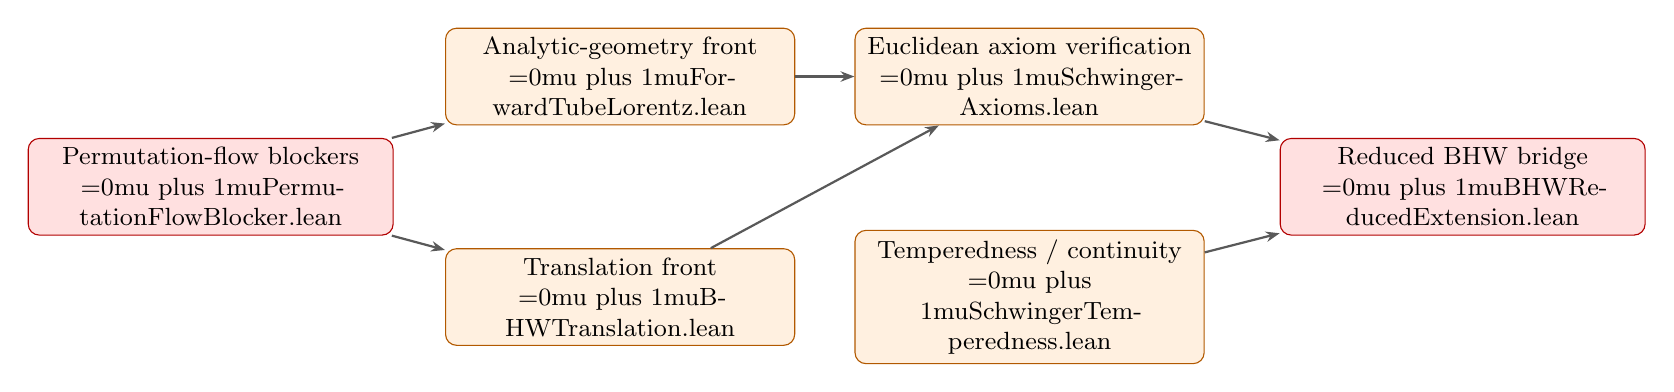
\begin{tikzpicture}[
  flagged/.style={rectangle, rounded corners, draw=orange!70!black, fill=orange!12,
    text width=4.2cm, minimum height=1.15cm, align=center, font=\small},
  upstream/.style={rectangle, rounded corners, draw=red!70!black, fill=red!12,
    text width=4.4cm, minimum height=1.15cm, align=center, font=\small},
  arr/.style={-{Stealth[length=5pt]}, thick, gray!70!black},
]
\node[upstream] (perm) at (0,0)
  {Permutation-flow blockers\\\leanfile{PermutationFlowBlocker.lean}};
\node[flagged] (ftl) at (5.2,1.4)
  {Analytic-geometry front\\\leanfile{ForwardTubeLorentz.lean}};
\node[flagged] (bhw) at (5.2,-1.4)
  {Translation front\\\leanfile{BHWTranslation.lean}};
\node[flagged] (sax) at (10.4,1.4)
  {Euclidean axiom verification\\\leanfile{SchwingerAxioms.lean}};
\node[flagged] (stem) at (10.4,-1.4)
  {Temperedness / continuity\\\leanfile{SchwingerTemperedness.lean}};
\node[upstream] (red) at (15.9,0)
  {Reduced BHW bridge\\\leanfile{BHWReducedExtension.lean}};
\draw[arr] (perm) -- (ftl);
\draw[arr] (perm) -- (bhw);
\draw[arr] (ftl) -- (sax);
\draw[arr] (bhw) -- (sax);
\draw[arr] (stem) -- (red);
\draw[arr] (sax) -- (red);
\end{tikzpicture}
\end{adjustbox}

\medskip
\textbf{Flow chart:} flagged $R \to E$ blocker map (not current implementation focus).
\end{center}

\subsection{GNS Construction}

\begin{center}
\begin{adjustbox}{max width=0.84\textwidth,center}
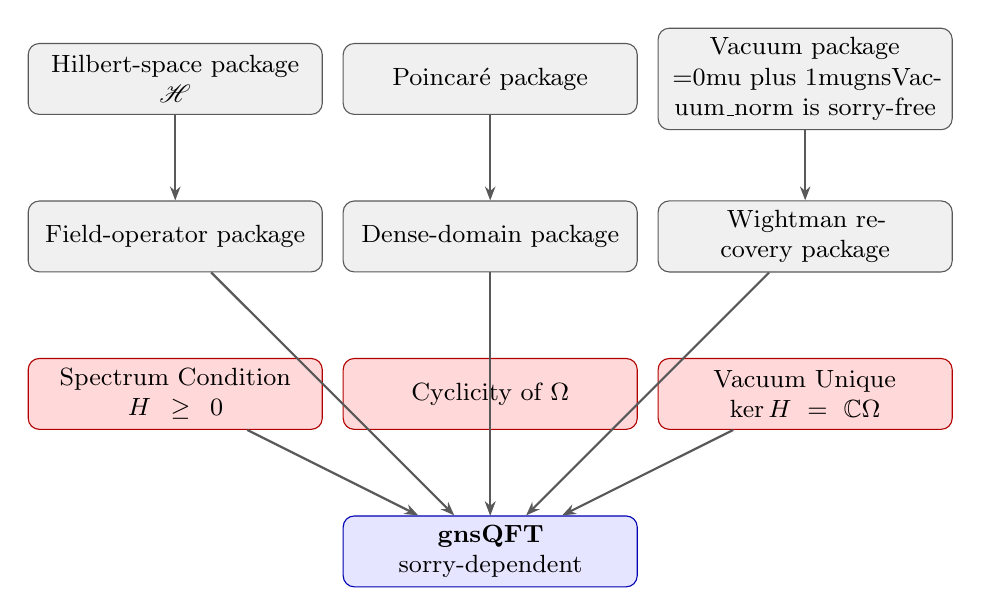
\begin{tikzpicture}[
  package/.style={rectangle, rounded corners, draw=gray!70!black, fill=gray!12,
    text width=3.5cm, minimum height=0.9cm, align=center, font=\small},
  dep/.style={rectangle, rounded corners, draw=blue!70!black, fill=blue!10,
    text width=3.5cm, minimum height=0.9cm, align=center, font=\small},
  sorry/.style={rectangle, rounded corners, draw=red!70!black, fill=red!15,
    text width=3.5cm, minimum height=0.9cm, align=center, font=\small},
  arr/.style={-{Stealth[length=5pt]}, thick, gray!70!black},
]
\node[package] (hilbert) at (0, 4) {Hilbert-space package\\$\mathscr{H}$};
\node[package] (poincare) at (4, 4) {Poincar\'e package};
\node[package] (vacuum) at (8, 4) {Vacuum package\\\leanname{gnsVacuum\_norm} is sorry-free};
\node[package] (field) at (0, 2) {Field-operator package};
\node[package] (domain) at (4, 2) {Dense-domain package};
\node[package] (wightman) at (8, 2) {Wightman recovery package};
\node[sorry] (spectrum) at (0, 0) {Spectrum Condition\\$H \geq 0$};
\node[sorry] (cyclic) at (4, 0) {Cyclicity of $\Omega$};
\node[sorry] (unique) at (8, 0) {Vacuum Unique\\$\ker H = \mathbb{C}\Omega$};
\node[dep] (gns) at (4, -2) {\textbf{gnsQFT}\\sorry-dependent};
\draw[arr] (hilbert) -- (field); \draw[arr] (poincare) -- (domain);
\draw[arr] (vacuum) -- (wightman);
\draw[arr] (field) -- (gns); \draw[arr] (domain) -- (gns);
\draw[arr] (wightman) -- (gns);
\draw[arr] (spectrum) -- (gns); \draw[arr] (cyclic) -- (gns);
\draw[arr] (unique) -- (gns);
\end{tikzpicture}
\end{adjustbox}

\medskip
\textbf{Flow chart:} GNS construction. Gray nodes are established packages, the
blue node is a declaration that currently has sorry dependence, and the three red
nodes are the still-open externalized hypotheses of \leanname{gnsQFT}.
\end{center}

\subsection{Repository-wide Proof Structure Maps}

The two critical-path charts above show where progress is bottlenecked. The three
maps below are broader: they show how the main theorem packages in the current
repo fit together, including sorry-free declarations, sorry-dependent declarations,
explicit open theorems, and axioms.

\begin{center}
\begin{adjustbox}{max width=\textwidth,center}
\begin{tikzpicture}[
  sfree/.style={rectangle, rounded corners, draw=green!70!black, fill=green!12,
    text width=3.55cm, minimum height=1.0cm, align=center, font=\footnotesize},
  sdep/.style={rectangle, rounded corners, draw=blue!70!black, fill=blue!10,
    text width=3.55cm, minimum height=1.0cm, align=center, font=\footnotesize},
  open/.style={rectangle, rounded corners, draw=red!70!black, fill=red!12,
    text width=3.55cm, minimum height=1.0cm, align=center, font=\footnotesize},
  axiomnode/.style={rectangle, rounded corners, draw=orange!70!black, fill=orange!12,
    text width=3.55cm, minimum height=1.0cm, align=center, font=\footnotesize},
  package/.style={rectangle, rounded corners, draw=gray!70!black, fill=gray!12,
    text width=3.55cm, minimum height=1.0cm, align=center, font=\footnotesize},
  arr/.style={-{Stealth[length=4pt]}, thick, gray!70!black},
]
\node[package] (osh) at (0,0) {OS Hilbert package\\\leanfile{SchwingerOS.lean}};
\node[sfree] (semi) at (4.2,0) {\leanname{osTimeShiftHilbert}\\sorry-free};
\node[sdep] (holo) at (8.4,0) {\leanname{full\_analytic\_continuation}\\proved, sorry-dependent};
\node[package] (k2b) at (12.6,0) {$k=2$ support package\\{\footnotesize\texttt{OSToWightmanK2}\\\texttt{BaseStep.lean}}};
\node[open] (vi1a) at (16.8,1.25) {VI.1 sequence limit\\negative approx.-identity};
\node[open] (vi1b) at (16.8,-1.25) {Final $k=2$ assembly\\distributional package};
\node[sdep] (k2main) at (21.0,0) {\leanname{schwinger\_continuation\_base\_step\_timeParametric\_k2}\\proved, sorry-dependent};
\node[open] (genk) at (25.2,0) {\leanfile{OSToWightman.lean}\\2 private open theorems};
\node[sdep] (bv) at (29.4,0) {\leanname{boundary\_values\_tempered}\\proved, sorry-dependent};
\node[sdep] (mainer) at (33.6,0) {\leanname{os\_to\_wightman}\\proved, sorry-dependent};
\draw[arr] (osh) -- (semi);
\draw[arr] (semi) -- (holo);
\draw[arr] (holo) -- (k2b);
\draw[arr] (k2b) -- (vi1a);
\draw[arr] (k2b) -- (vi1b);
\draw[arr] (vi1a) -- (k2main);
\draw[arr] (vi1b) -- (k2main);
\draw[arr] (k2main) -- (genk);
\draw[arr] (genk) -- (bv);
\draw[arr] (bv) -- (mainer);
\end{tikzpicture}
\end{adjustbox}

\medskip
\textbf{Structure map:} repo-wide $E \to R$ theorem structure.
\end{center}

\noindent
In the $E \to R$ chart, the two red VI.1 nodes abbreviate the full theorem names
\leanname{translatedProductShell\_boundary\_tendsto\_schwingerDifferencePositive\_of\_negativeApproxIdentity\_local}
and \leanname{exists\_k2\_timeParametric\_distributional\_assembly}.

\begin{center}
\begin{adjustbox}{max width=\textwidth,center}
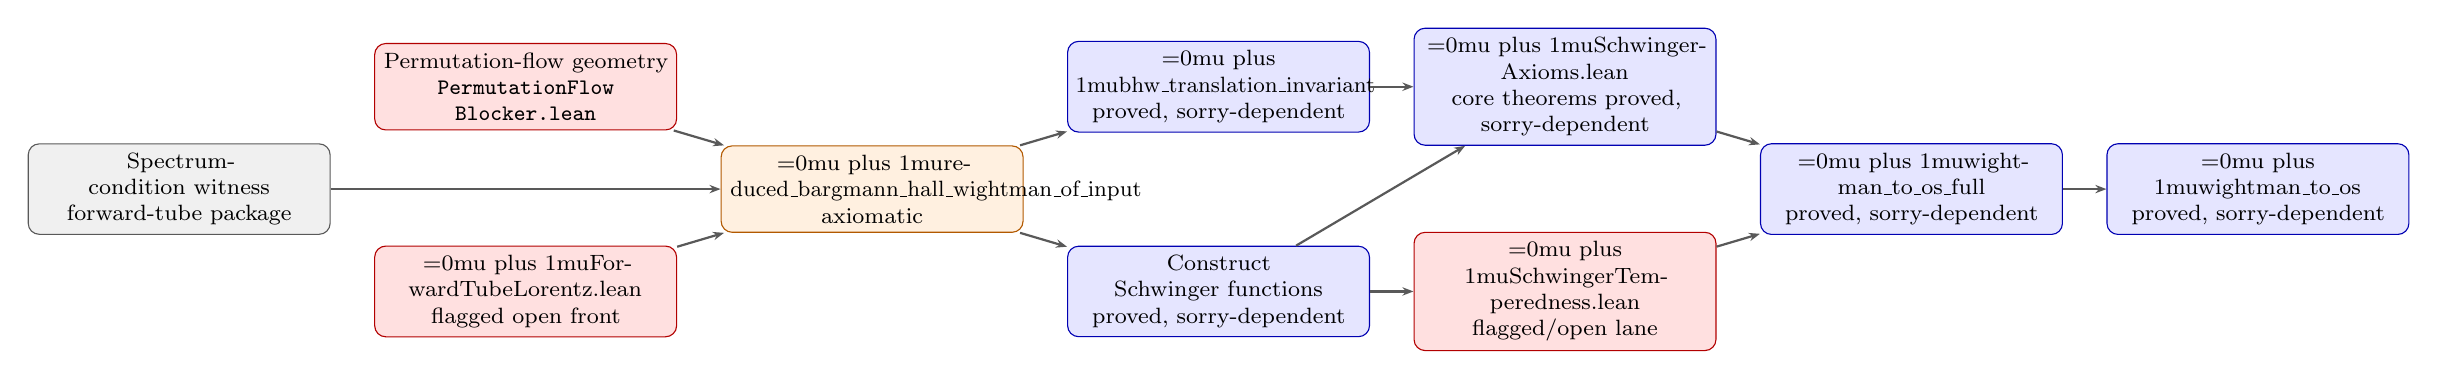
\begin{tikzpicture}[
  sfree/.style={rectangle, rounded corners, draw=green!70!black, fill=green!12,
    text width=3.6cm, minimum height=1.0cm, align=center, font=\footnotesize},
  sdep/.style={rectangle, rounded corners, draw=blue!70!black, fill=blue!10,
    text width=3.6cm, minimum height=1.0cm, align=center, font=\footnotesize},
  open/.style={rectangle, rounded corners, draw=red!70!black, fill=red!12,
    text width=3.6cm, minimum height=1.0cm, align=center, font=\footnotesize},
  axiomnode/.style={rectangle, rounded corners, draw=orange!70!black, fill=orange!12,
    text width=3.6cm, minimum height=1.0cm, align=center, font=\footnotesize},
  package/.style={rectangle, rounded corners, draw=gray!70!black, fill=gray!12,
    text width=3.6cm, minimum height=1.0cm, align=center, font=\footnotesize},
  arr/.style={-{Stealth[length=4pt]}, thick, gray!70!black},
]
\node[package] (spec) at (0,0) {Spectrum-condition witness\\forward-tube package};
\node[open] (perm) at (4.4,1.3) {Permutation-flow geometry\\{\footnotesize\texttt{PermutationFlow}\\\texttt{Blocker.lean}}};
\node[open] (ftl) at (4.4,-1.3) {\leanfile{ForwardTubeLorentz.lean}\\flagged open front};
\node[axiomnode] (bhwaxiom) at (8.8,0) {\leanname{reduced\_bargmann\_hall\_wightman\_of\_input}\\axiomatic};
\node[sdep] (bhwtrans) at (13.2,1.3) {\leanname{bhw\_translation\_invariant}\\proved, sorry-dependent};
\node[sdep] (schfns) at (13.2,-1.3) {Construct Schwinger functions\\proved, sorry-dependent};
\node[sdep] (sax) at (17.6,1.3) {\leanfile{SchwingerAxioms.lean}\\core theorems proved, sorry-dependent};
\node[open] (stem) at (17.6,-1.3) {\leanfile{SchwingerTemperedness.lean}\\flagged/open lane};
\node[sdep] (rfull) at (22.0,0) {\leanname{wightman\_to\_os\_full}\\proved, sorry-dependent};
\node[sdep] (rmain) at (26.4,0) {\leanname{wightman\_to\_os}\\proved, sorry-dependent};
\draw[arr] (spec) -- (bhwaxiom);
\draw[arr] (perm) -- (bhwaxiom);
\draw[arr] (ftl) -- (bhwaxiom);
\draw[arr] (bhwaxiom) -- (bhwtrans);
\draw[arr] (bhwaxiom) -- (schfns);
\draw[arr] (bhwtrans) -- (sax);
\draw[arr] (schfns) -- (sax);
\draw[arr] (schfns) -- (stem);
\draw[arr] (sax) -- (rfull);
\draw[arr] (stem) -- (rfull);
\draw[arr] (rfull) -- (rmain);
\end{tikzpicture}
\end{adjustbox}

\medskip
\textbf{Structure map:} repo-wide $R \to E$ theorem structure.
\end{center}

\begin{center}
\begin{adjustbox}{max width=0.95\textwidth,center}
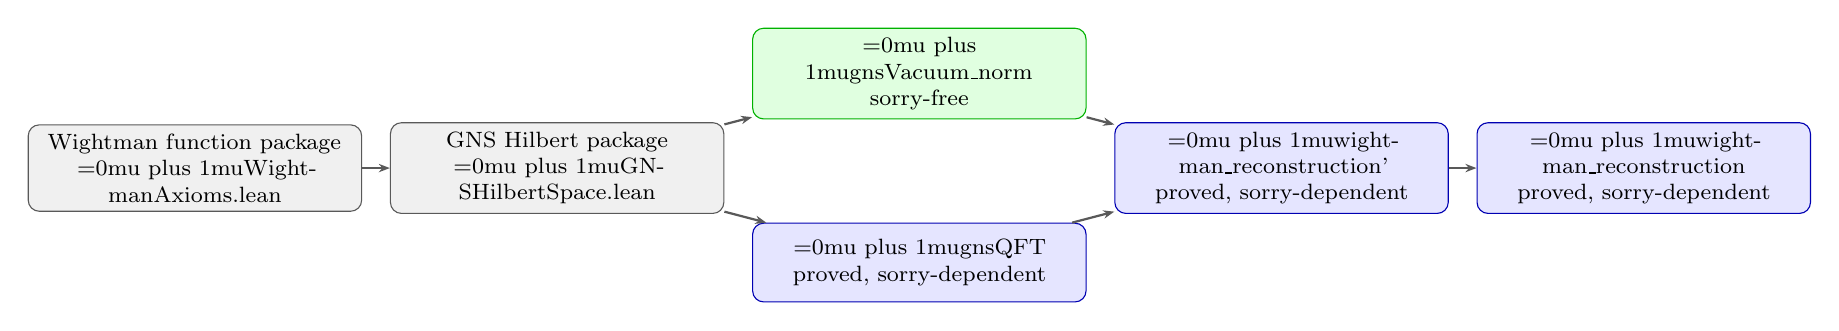
\begin{tikzpicture}[
  sfree/.style={rectangle, rounded corners, draw=green!70!black, fill=green!12,
    text width=4.0cm, minimum height=1.0cm, align=center, font=\footnotesize},
  sdep/.style={rectangle, rounded corners, draw=blue!70!black, fill=blue!10,
    text width=4.0cm, minimum height=1.0cm, align=center, font=\footnotesize},
  open/.style={rectangle, rounded corners, draw=red!70!black, fill=red!12,
    text width=4.0cm, minimum height=1.0cm, align=center, font=\footnotesize},
  package/.style={rectangle, rounded corners, draw=gray!70!black, fill=gray!12,
    text width=4.0cm, minimum height=1.0cm, align=center, font=\footnotesize},
  arr/.style={-{Stealth[length=4pt]}, thick, gray!70!black},
]
\node[package] (wfn) at (0,0) {Wightman function package\\\leanfile{WightmanAxioms.lean}};
\node[package] (ghilb) at (4.6,0) {GNS Hilbert package\\\leanfile{GNSHilbertSpace.lean}};
\node[sfree] (gvac) at (9.2,1.2) {\leanname{gnsVacuum\_norm}\\sorry-free};
\node[sdep] (gqft) at (9.2,-1.2) {\leanname{gnsQFT}\\proved, sorry-dependent};
\node[sdep] (wrec) at (13.8,0) {\leanname{wightman\_reconstruction'}\\proved, sorry-dependent};
\node[sdep] (mrec) at (18.4,0) {\leanname{wightman\_reconstruction}\\proved, sorry-dependent};
\draw[arr] (wfn) -- (ghilb);
\draw[arr] (ghilb) -- (gvac);
\draw[arr] (ghilb) -- (gqft);
\draw[arr] (gvac) -- (wrec);
\draw[arr] (gqft) -- (wrec);
\draw[arr] (wrec) -- (mrec);
\end{tikzpicture}
\end{adjustbox}

\medskip
\textbf{Structure map:} standalone GNS/Wightman reconstruction lane.
\end{center}

\noindent
\textbf{Chart legend.} Green nodes are sorry-free declarations, blue nodes are
proved declarations with sorry/axiom dependence, red nodes are explicit open
theorems, orange nodes are axioms, and gray nodes are support packages or
definition-level bundles rather than single theorem claims.


%% ===================================================================
\part{The Axiom Systems}
%% ===================================================================

\section{Euclidean Axioms (OS~I, Section~3)}

The Euclidean Green's functions (Schwinger functions) $\{\mathfrak{S}_n\}_{n=0}^\infty$
are distributions on the $n$-point configuration space, restricted to the
``zero-diagonal'' subspace (test functions vanishing to infinite order when any two
points coincide). The axioms are:

\begin{description}[leftmargin=2cm]
\item[(E0)] \textbf{Temperedness.}
  $\mathfrak{S}_0 \equiv 1$, each $\mathfrak{S}_n$ is a continuous linear
  functional on the zero-diagonal Schwartz space.

\item[(E0')] \textbf{Linear growth condition} (OS~II).
  The distributional order of $\mathfrak{S}_n$ grows at most linearly in $n$.

\item[(E1)] \textbf{Euclidean covariance.}
  $\mathfrak{S}_n(f_{(a,R)}) = \mathfrak{S}_n(f)$ for all $SO(d{+}1)$ rotations
  $R$ and translations $a$.

\item[(E2)] \textbf{Reflection positivity.}
  The sesquilinear form
  $\sum_{n,m} \mathfrak{S}_{n+m}(\Theta f_n^* \times f_m) \geq 0$
  for all positive-time test sequences.

\item[(E3)] \textbf{Permutation symmetry.}
  $\mathfrak{S}_n(f) = \mathfrak{S}_n(f^\pi)$ for all permutations $\pi$.

\item[(E4)] \textbf{Cluster property.}
  $\mathfrak{S}_{n+m}(f \times g_{\lambda a}) \to
  \mathfrak{S}_n(f) \cdot \mathfrak{S}_m(g)$ as $\lambda \to \infty$.
\end{description}

\medskip
In Lean, these are bundled into a single structure. The \leanname{SchwingerFunctions}
type is $\texttt{(n : } \mathbb{N}\texttt{) } \to \texttt{ZeroDiagonalSchwartz d n} \to \mathbb{C}$,
where $\texttt{ZeroDiagonalSchwartz d n}$ is the subtype of $n$-point Schwartz functions
that vanish to infinite order on the coincidence set $\{x \mid x_i = x_j \text{ for some } i \neq j\}$.

\begin{lstlisting}
-- SchwingerOS.lean:721
structure OsterwalderSchraderAxioms (d : N) [NeZero d] where
  S : SchwingerFunctions d
  E0_tempered : forall n, Continuous (S n)
  E0_linear : forall n, IsLinearMap C (S n)
  E0_reality : forall (n : N) (f g : ZeroDiagonalSchwartz d n),
    (forall x, g.1 x = starRingEnd C (f.1 (timeReflectionN d x))) ->
    starRingEnd C (S n f) = S n g
  E1_translation_invariant : forall (n : N) (a : SpacetimeDim d)
    (f g : ZeroDiagonalSchwartz d n),
    (forall x, g.1 x = f.1 (fun i => x i + a)) ->
    S n f = S n g
  E1_rotation_invariant : forall (n : N)
    (R : Matrix (Fin (d+1)) (Fin (d+1)) R),
    R.transpose * R = 1 -> R.det = 1 ->
    forall (f g : ZeroDiagonalSchwartz d n),
    (forall x, g.1 x = f.1 (fun i => R.mulVec (x i))) ->
    S n f = S n g
  E2_reflection_positive : forall (F : BorchersSequence d),
    (forall n, tsupport ((F.funcs n : SchwartzNPoint d n) :
      NPointDomain d n -> C) <=
      OrderedPositiveTimeRegion d n) ->
    (OSInnerProduct d S F F).re >= 0
  E3_symmetric : forall (n : N) (sigma : Equiv.Perm (Fin n))
    (f g : ZeroDiagonalSchwartz d n),
    (forall x, g.1 x = f.1 (fun i => x (sigma i))) ->
    S n f = S n g
  E4_cluster : forall (n m : N) (f : ZeroDiagonalSchwartz d n)
    (g : ZeroDiagonalSchwartz d m),
    forall eps : R, eps > 0 -> exists R0 : R, R0 > 0 /\
      forall a : SpacetimeDim d, a 0 = 0 ->
        (∑ i : Fin d, (a (Fin.succ i))^2) > R0^2 ->
        forall (g_a : ZeroDiagonalSchwartz d m),
          (forall x : NPointDomain d m,
            g_a.1 x = g.1 (fun i => x i - a)) ->
          forall (fg_a : ZeroDiagonalSchwartz d (n + m)),
            (forall x : NPointDomain d (n + m),
              fg_a.1 x =
                f.1 (splitFirst n m x) * g_a.1 (splitLast n m x)) ->
            norm (S (n + m) fg_a - S n f * S m g) < eps
\end{lstlisting}

\noindent\textbf{Mathematical meaning of each field:}
\begin{itemize}
\item \texttt{S}: the sequence of $n$-point Schwinger functions, each a
  complex-valued functional on zero-diagonal Schwartz $n$-point test functions.
\item \texttt{E0\_tempered}, \texttt{E0\_linear}: each $\mathfrak{S}_n$ is a
  continuous linear functional (tempered distribution) on the zero-diagonal
  Schwartz space.
\item \texttt{E0\_reality}: the reality condition
  $\overline{\mathfrak{S}_n(f)} = \mathfrak{S}_n(\overline{f \circ \Theta})$
  where $\Theta$ is time reflection.
\item \texttt{E1\_translation\_invariant}: $\mathfrak{S}_n$ is invariant under
  simultaneous translation of all $n$ points by any vector $a$.
\item \texttt{E1\_rotation\_invariant}: $\mathfrak{S}_n$ is invariant under
  simultaneous $SO(d{+}1)$ rotation $R$ of all $n$ points.
\item \texttt{E2\_reflection\_positive}: for any positive-time Borchers sequence
  $F$ (a finite sequence of test functions supported in the ordered positive-time
  region), the OS inner product $(F, F) \geq 0$.
\item \texttt{E3\_symmetric}: $\mathfrak{S}_n$ is invariant under permutation
  of the $n$ points.
\item \texttt{E4\_cluster}: the connected correlation vanishes at spacelike
  infinity.
\end{itemize}

\subsection{The Linear Growth Condition (OS~II, Section~IV.1)}

OS~II replaces the temperedness axiom E0 with the stronger \emph{linear growth
condition} E0': the distributional order of $\mathfrak{S}_n$ grows at most
linearly in $n$, with factorial-growth constants.

\begin{lstlisting}
-- SchwingerOS.lean:1816
structure OSLinearGrowthCondition (d : N) [NeZero d]
    (OS : OsterwalderSchraderAxioms d) where
  normalized_zero : forall f : ZeroDiagonalSchwartz d 0,
    OS.S 0 f = f.1 0
  sobolev_index : N
  alpha : R
  beta : R
  gamma : R
  alpha_pos : alpha > 0
  beta_pos : beta > 0
  growth_estimate : forall (n : N) (f : ZeroDiagonalSchwartz d n),
    norm (OS.S n f) <=
      alpha * beta ^ n * (n.factorial : R) ^ gamma *
        SchwartzMap.seminorm R sobolev_index sobolev_index f.1
\end{lstlisting}

\noindent\textbf{Mathematical meaning:}
The bound $|\mathfrak{S}_n(f)| \leq \alpha \beta^n (n!)^\gamma |f|_s$
says the $n$-point function is controlled by a single Schwartz seminorm
$|f|_s$ (with the \emph{same} Sobolev index $s$ for all $n$), times a
factorial growth factor. This is the key input for the temperedness
estimates in OS~II Section~VI.

\section{Wightman Axioms (OS~I, p.~88)}

The Wightman distributions $\{\mathfrak{W}_n\}$ satisfy:
R0 (temperedness), R1 (Poincar\'e invariance), R2 (positivity),
R3 (local commutativity), R4 (cluster property), R5 (spectral condition).

In Lean, these are bundled into the \leanname{WightmanQFT} structure, which
packages a Hilbert space $\mathscr{H}$, a Poincar\'e representation, a vacuum
vector, operator-valued distributions (field operators), and all the axiom
properties.

\begin{lstlisting}
-- WightmanAxioms.lean:138
structure WightmanQFT (d : N) [NeZero d] where
  HilbertSpace : Type*
  [instNormedAddCommGroup : NormedAddCommGroup HilbertSpace]
  [instInnerProductSpace : InnerProductSpace C HilbertSpace]
  [instCompleteSpace : CompleteSpace HilbertSpace]
  poincare_rep : PoincareRepresentation d HilbertSpace
  spectrum_condition : SpectralCondition d poincare_rep
  vacuum : HilbertSpace
  vacuum_normalized : norm vacuum = 1
  vacuum_invariant : IsPoincareInvariant poincare_rep vacuum
  field : OperatorValuedDistribution d HilbertSpace
  vacuum_in_domain : vacuum mem field.domain
  field_hermitian : forall (f : SchwartzSpacetime d) (chi psi),
    chi mem field.domain -> psi mem field.domain ->
    inner (field.operator f chi) psi =
      inner chi (field.operator (SchwartzMap.conj f) psi)
  cyclicity : Dense (field.algebraicSpan vacuum).carrier
  covariance : ∀ (g : PoincareGroup d) (f : SchwartzSpacetime d)
    (χ ψ : HilbertSpace),
    χ mem field.domain -> ψ mem field.domain ->
    inner (poincare_rep.U g χ) (field.operator f (poincare_rep.U g ψ)) =
      inner χ (field.operator (poincareActionOnSchwartz g⁻¹ f) ψ)
  locality : IsLocal d field
  vacuum_unique : VacuumUnique d poincare_rep vacuum
\end{lstlisting}

\noindent\textbf{Mathematical meaning of key fields:}
\begin{itemize}
\item \texttt{HilbertSpace}: the physical Hilbert space $\mathscr{H}$ carrying
  the quantum field theory.
\item \texttt{poincare\_rep}: a continuous unitary representation of the
  Poincar\'e group on $\mathscr{H}$.
\item \texttt{spectrum\_condition}: the joint spectrum of the energy-momentum
  operators lies in the closed forward light cone $\overline{V}_+$.
\item \texttt{vacuum}: a unit vector $\Omega \in \mathscr{H}$ invariant under
  all Poincar\'e transformations.
\item \texttt{field}: an operator-valued tempered distribution
  $\phi : \Schwartz(\mathbb{R}^{d+1}) \to \mathrm{Op}(\mathscr{D}_0, \mathscr{H})$
  mapping test functions to (unbounded) operators on a dense domain $\mathscr{D}_0$.
\item \texttt{field\_hermitian}: $\langle \phi(f)\chi, \psi \rangle =
  \langle \chi, \phi(\bar{f})\psi \rangle$ (the field is hermitian/real).
\item \texttt{cyclicity}: the set $\{\phi(f_1)\cdots\phi(f_n)\Omega\}$ is
  dense in $\mathscr{H}$ (the vacuum is cyclic for the field algebra).
\item \texttt{locality}: $[\phi(f), \phi(g)] = 0$ when $f$ and $g$ have
  spacelike-separated supports (microcausality).
\item \texttt{vacuum\_unique}: $\Omega$ is the unique (up to phase)
  translation-invariant vector in $\mathscr{H}$.
\end{itemize}


%% ===================================================================
\part{Theorem E-to-R: Euclidean to Relativistic}
%% ===================================================================

\section{The OS Hilbert Space (OS~I, Section~4.1)}

\subsection{The OS Inner Product}

Given Schwinger functions $\mathfrak{S}_n$ satisfying E0 and E2, one defines
a positive semi-definite sesquilinear form on the space of positive-time
Borchers sequences:

\begin{definition}[OS Inner Product, OS~I eq.~(4.3)]
\[
(F, G) = \sum_{n,m} \mathfrak{S}_{n+m}(\Theta F_n^* \otimes G_m)
\]
where $\Theta$ denotes time reflection and ${}^*$ denotes complex conjugation.
\end{definition}

\begin{lstlisting}
-- SchwingerOS.lean:26
-- Computes the OS inner product by summing over all pairs
-- of components in the Borchers sequences F and G.
-- Each term applies OS.S to the osConj tensor product of the
-- n-th component of F with the m-th component of G.
def OSInnerProduct (S : SchwingerFunctions d)
    (F G : BorchersSequence d) : C :=
  Finset.sum (Finset.range (F.bound + 1)) fun n =>
    Finset.sum (Finset.range (G.bound + 1)) fun m =>
      S (n + m) (ZeroDiagonalSchwartz.ofClassical
        ((F.funcs n).osConjTensorProduct (G.funcs m)))
\end{lstlisting}

\noindent Here \texttt{osConjTensorProduct} applies time-reflected complex
conjugation to the left factor $F_n$, then forms the tensor product with $G_m$,
yielding an $(n{+}m)$-point test function in the zero-diagonal Schwartz space.

\begin{theorem}[One-point reduction, SchwingerOS.lean:429]
For one-point Borchers sequences $F = \mathrm{single}(n, f)$ and
$G = \mathrm{single}(m, g)$:
\[
(F, G) = \mathfrak{S}_{n+m}\bigl(\mathrm{ofClassical}(f.\mathrm{osConjTensorProduct}\,g)\bigr).
\]
\end{theorem}

\begin{lstlisting}
-- SchwingerOS.lean:429 (PROVED)
-- Reduces the full Borchers inner product to a single
-- Schwinger function evaluation when both sequences are
-- supported in a single degree.
theorem OSInnerProduct_single_single
    (S : (n : N) -> ZeroDiagonalSchwartz d n -> C)
    (hlin : forall n, IsLinearMap C (S n))
    (n m : N) (f : SchwartzNPoint d n) (g : SchwartzNPoint d m) :
    OSInnerProduct d S (BorchersSequence.single n f)
      (BorchersSequence.single m g) =
      S (n + m) (ZeroDiagonalSchwartz.ofClassical
        (f.osConjTensorProduct g))
\end{lstlisting}

\subsection{The Pre-Hilbert Space and Completion}

The OS pre-Hilbert space is the quotient of the positive-time Borchers
algebra by the null space of the inner product:
\[
\mathscr{H}_0 = \mathscr{L}_+ / \mathscr{N},
\qquad
\mathscr{N} = \{F \in \mathscr{L}_+ : (F, F) = 0\}.
\]
The Hilbert space $\mathscr{H}$ is the completion of $\mathscr{H}_0$.

\begin{lstlisting}
-- SchwingerOS.lean:2109
-- The OS pre-Hilbert space: quotient of positive-time Borchers
-- sequences by the equivalence relation identifying sequences
-- whose difference has zero OS inner product with everything.
def OSPreHilbertSpace (OS : OsterwalderSchraderAxioms d) : Type :=
  Quotient (osBorchersSetoid OS)
\end{lstlisting}

The inner product properties are established in \leanfile{SchwingerOS.lean}. The
display below records the source-level theorem surfaces; this subsection is not
claiming an individual dependency audit for each one:

\begin{lstlisting}
-- SchwingerOS.lean (ALL PROVED)
-- Hermitian symmetry: <y, x> = conj(<x, y>)
theorem inner_conj_symm (x y : OSPreHilbertSpace OS) :
    starRingEnd C (inner y x) = inner x y

-- Positive semi-definiteness: Re(<x, x>) >= 0
theorem inner_re_nonneg (x : OSPreHilbertSpace OS) :
    0 <= (inner x x).re

-- Linearity in the first argument
theorem inner_add_left (x y z : OSPreHilbertSpace OS) :
    inner (x + y) z = inner x z + inner y z

-- Scalar multiplication
theorem inner_smul_left (c : C) (x y : OSPreHilbertSpace OS) :
    inner (c smul x) y = starRingEnd C c * inner x y

-- Definiteness: <x, x> = 0 implies x = 0
theorem inner_definite (x : OSPreHilbertSpace OS) :
    inner x x = 0 -> x = 0
\end{lstlisting}

\medskip\noindent
At the level relevant for the current route audit, the important point is that
\leanname{OSInnerProduct} itself is a sorry-free definition and the pre-Hilbert
package built on top of it is stable infrastructure, not a current source of
critical-path \sorry{}s.


\section{The Contraction Semigroup (OS~I, pp.~91--92)}

From E0, E1, and E2, one constructs a time-translation semigroup
$\{T^t\}_{t \geq 0}$ on $\mathscr{H}$ satisfying:
\begin{itemize}
\item $T^0 = \mathrm{id}$ (initial condition),
\item $T^{s+t} = T^s \circ T^t$ (semigroup law),
\item $\|T^t x\| \leq \|x\|$ (contraction property),
\item $\mathrm{Re}\langle x, T^t x \rangle \geq 0$ (positivity).
\end{itemize}

\begin{lstlisting}
-- OSToWightmanSemigroup.lean:60
-- The Euclidean time-translation semigroup on the OS
-- pre-Hilbert space, satisfying contraction, positivity,
-- and the semigroup composition law.
structure EuclideanSemigroup (OS : OsterwalderSchraderAxioms d) where
  T : (t : R) -> (ht : 0 < t) ->
    OSPreHilbertSpace OS ->L[C] OSPreHilbertSpace OS
  semigroup : forall s t hs ht,
    (T s hs).comp (T t ht) = T (s + t) (add_pos hs ht)
  contraction : forall t ht x, norm ((T t ht) x) <= norm x
  positive : forall t ht x,
    0 <= RCLike.re (inner x ((T t ht) x))
\end{lstlisting}

\noindent\textbf{Mathematical meaning:} The contraction semigroup $T^t$ encodes
Euclidean time evolution. The contraction property $\|T^t\| \leq 1$ follows from
the Cauchy--Schwarz inequality applied to the OS inner product (OS~I, eq.~(4.9)).
The generator $H = -\log T^1$ is a positive self-adjoint operator (the Hamiltonian),
and $T^t = e^{-tH}$ for $t \geq 0$.

\medskip\noindent
\textbf{Dependency-aware status.}
Direct audit shows that \leanname{osTimeShiftHilbert} is currently sorry-free.
So the semigroup core itself is not a live frontier. The active dependence on
open work only reappears later, when these semigroup matrix elements are
assembled into full continuation theorems.

\subsection{The Complex Semigroup}

The semigroup extends holomorphically to $\{\tau \in \mathbb{C} : \mathrm{Re}\,\tau > 0\}$
via the spectral functional calculus:

\begin{lstlisting}
-- OSToWightmanSemigroup.lean:3047
-- The complex semigroup T^tau for Re(tau) > 0, constructed
-- via the spectral functional calculus applied to the
-- generator T(1) (a positive self-adjoint contraction).
def osTimeShiftHilbertComplex
    (OS : OsterwalderSchraderAxioms d)
    (lgc : OSLinearGrowthCondition d OS) (z : C) :
    OSHilbertSpace OS ->L[C] OSHilbertSpace OS :=
  ContinuousLinearMap.spectralSemigroupComplex
    (osTimeShiftHilbert OS lgc 1 one_pos)
    (osTimeShiftHilbert_isSelfAdjoint OS lgc 1 one_pos)
    (osTimeShiftHilbert_nonneg OS lgc 1 one_pos)
    (spectrum_osTimeShiftHilbert_subset_Icc OS lgc 1 one_pos)
    z
\end{lstlisting}

\begin{lstlisting}
-- OSToWightmanSemigroup.lean:3074 (PROVED)
-- The matrix element <x, T(z) y> is holomorphic in z
-- on the right half-plane {Re z > 0}.
theorem differentiableOn_inner_osTimeShiftHilbertComplex
    (OS : OsterwalderSchraderAxioms d)
    (lgc : OSLinearGrowthCondition d OS)
    (x y : OSHilbertSpace OS) :
    DifferentiableOn C
      (fun z => inner x
        (osTimeShiftHilbertComplex OS lgc z y))
      {z : C | 0 < z.re}
\end{lstlisting}

\noindent This holomorphicity is the foundation for the analytic continuation
of the Schwinger functions from real Euclidean time to complex time, and
ultimately to Minkowski spacetime.

\medskip\noindent
\textbf{Dependency-aware status.}
The displayed matrix-element theorem
\leanname{differentiableOn\_inner\_osTimeShiftHilbertComplex} is also
sorry-free in direct audit. So the holomorphic one-variable semigroup layer is
genuinely closed support infrastructure in the current repo.


\section{Spatial Translations (OS~I, p.~91)}

From E1, spatial translations extend to a strongly continuous unitary group
$U_s(a)$ on $\mathscr{H}$:

\begin{lstlisting}
-- OSToWightmanSpatialMomentum.lean:565
-- The spatial translation unitary group on the OS Hilbert space.
-- U_s(a) translates all points by a in the spatial directions.
noncomputable def osSpatialTranslateHilbert
    (OS : OsterwalderSchraderAxioms d) (a : Fin d -> R) :
    OSHilbertSpace OS ->L[C] OSHilbertSpace OS

-- Line 645 (PROVED): composition law U(a) . U(b) = U(a+b)
theorem osSpatialTranslateHilbert_comp (OS) (a b) :
    (osSpatialTranslateHilbert OS a).comp
      (osSpatialTranslateHilbert OS b) =
    osSpatialTranslateHilbert OS (a + b)
\end{lstlisting}

\medskip\noindent
\textbf{Dependency-aware status.}
Direct audit shows that \leanname{osSpatialTranslateHilbert\_comp} is
sorry-free. This matters because the current VI.1 route repeatedly packages
mixed time-translation and spatial-translation orbits, so it is useful to know
that the spatial group law itself is not part of the unresolved frontier.


\section{Analytic Continuation (OS~I, Section~4.1; OS~II, Section~V)}

The holomorphic semigroup enables analytic continuation of the Schwinger
functions in the time variables. OS~II uses an inductive procedure:
at step $r$, analytically continue $S_k$ from the real domain $\mathbb{R}^{4k}_+$
to the complex region $C_k^{(r)}$.

\begin{lstlisting}
-- OSToWightman.lean:1938 (PROVED)
-- The full analytic continuation: for each n, there exists
-- a holomorphic function F on the forward tube that equals
-- the Schwinger function on Euclidean real points.
theorem full_analytic_continuation
    (OS : OsterwalderSchraderAxioms d)
    (lgc : OSLinearGrowthCondition d OS)
    (k : N) :
    exists (W_analytic : (Fin k -> Fin (d+1) -> C) -> C),
      DifferentiableOn C W_analytic (ForwardTube d k) /\
      (forall (f : ZeroDiagonalSchwartz d k),
        OS.S k f = ∫ x : NPointDomain d k,
          W_analytic (fun j => wickRotatePoint (x j)) * (f.1 x))
\end{lstlisting}

\begin{lstlisting}
-- OSToWightman.lean:1903 (PROVED)
-- The inductive step: extend from C_k^(r) to C_k^(r+1).
theorem iterated_analytic_continuation
    (OS : OsterwalderSchraderAxioms d)
    (lgc : OSLinearGrowthCondition d OS)
    (k : N) :
    exists (S_ext : (Fin k -> Fin (d+1) -> C) -> C),
      DifferentiableOn C S_ext
        (AnalyticContinuationRegion d k (d + 1)) /\
      (forall (f : ZeroDiagonalSchwartz d k),
        OS.S k f = ∫ x : NPointDomain d k,
          S_ext (fun j => wickRotatePoint (x j)) * (f.1 x))
\end{lstlisting}

\medskip\noindent
\textbf{Dependency-aware status.}
The main continuation theorems \leanname{full\_analytic\_continuation} and
\leanname{iterated\_analytic\_continuation} are both present in Lean, but direct
audit shows that they are currently \emph{sorry-dependent}. Mathematically, they
already express the right OS~I / OS~II theorem surfaces; formally, they still
inherit unresolved work from the later $k=2$, general-$k$, and boundary-value
layers.


\section{The k=2 Base Step (OS~II, Theorem~4.1)}

This is the initial nontrivial OS~II step on the corrected production route.
The repository now splits it into two files:
\begin{itemize}
\item \leanfile{OSToWightmanK2BaseStep.lean} --- the proved support layer:
  canonical probe witness, Bochner measure, positive-time shell identities,
  Laplace--Fourier reduction, and support/control lemmas.
\item \leanfile{OSToWightmanK2VI1.lean} --- the live OS~II Section~VI.1
  frontier: sequence-level regularization, boundary identification, and final
  existential $k=2$ assembly.
\end{itemize}

The public theorem surface is still the same $k=2$ base-step theorem, but the
remaining content is no longer described correctly as a fixed-probe kernel bound
plus shell-agreement theorem. The honest remaining gap is the sequence-level
VI.1 regularization limit.

\begin{lstlisting}[style=leansorry]
-- OSToWightmanK2VI1.lean:536
-- The public k=2 time-parametric base step.
theorem schwinger_continuation_base_step_timeParametric_k2
    (OS : OsterwalderSchraderAxioms d)
    (lgc : OSLinearGrowthCondition d OS) :
    exists (G : (Fin (2 * (d + 1)) -> C) -> C)
      (K : NPointDomain d 2 -> C),
      IsTimeHolomorphicFlatPositiveTimeDiffWitness G /\
      (forall x : NPointDomain d 2, x 0 0 < x 1 0 ->
        K x = k2TimeParametricKernel (d := d) G x) /\
      (forall x : NPointDomain d 2, x 1 0 < x 0 0 ->
        K x = k2TimeParametricKernel (d := d) G
          (fun i => x ((Equiv.swap (0 : Fin 2) (1 : Fin 2)) i))) /\
      (forall (f : ZeroDiagonalSchwartz d 2),
        OS.S 2 f =
          integral (fun x : NPointDomain d 2 => K x * (f.1 x)))
\end{lstlisting}

\noindent\textbf{Mathematical meaning:} There exist:
\begin{enumerate}
\item a time-holomorphic flattened witness $G$ on the positive-time-difference
  tube;
\item a genuine real Euclidean kernel $K$ on $NPointDomain\, d\, 2$ which agrees
  with the witness on the positive time-ordering sector and with the swapped
  witness on the negative sector;
\item a reproduction formula
  $\mathfrak{S}_2(f) = \int K(x)\, f(x)\, dx$
  for every zero-diagonal two-point Schwartz test.
\end{enumerate}

The theorem is still \textbf{open}, but its remaining content has been narrowed
to the honest VI.1 sequence-limit theorem and the final existential assembly
theorem above that limit.

\medskip\noindent
\textbf{Status summary.}
The public theorem
\leanname{schwinger\_continuation\_base\_step\_timeParametric\_k2} is still
\emph{open}. By contrast, \leanfile{OSToWightmanK2BaseStep.lean} is now a
compile-closed support file, while \leanfile{OSToWightmanK2VI1.lean} isolates
the two genuinely remaining VI.1 obligations.

\subsection{The Density Theorem}

A key ingredient is the density of ``flat-origin'' difference shells in
the zero-diagonal Schwartz space:

\begin{lstlisting}
-- OSToWightmanK2Density.lean (PROVED, 0 sorrys)
-- The C-span of difference lifts chi(u) . h(xi) with h
-- vanishing to infinite order at xi = 0 is dense in
-- ZeroDiagonalSchwartz d 2.
theorem flatOrigin_differenceShell_span_dense_zeroDiagonal :
    Dense (((Submodule.span C
      {f : ZeroDiagonalSchwartz d 2 |
        exists (chi h : SchwartzSpacetime d)
          (hzero : forall k : N,
            iteratedFDeriv R k (h : SpacetimeDim d -> C) 0 = 0),
          f = ZeroDiagonalSchwartz.ofClassical
            (twoPointDifferenceLift chi h)}) :
      Submodule C (ZeroDiagonalSchwartz d 2)) :
      Set (ZeroDiagonalSchwartz d 2))
\end{lstlisting}

\noindent\textbf{Mathematical meaning:} In center-difference coordinates
$(u, \xi) = (x_0, x_1 - x_0)$, a ``difference lift'' $\chi(u) h(\xi)$ is
a product tensor. The theorem says that such product tensors with $h$ flat
at the origin (all derivatives vanishing at $\xi = 0$) span a dense subspace
of the zero-diagonal test space. This enables extending kernel reproduction
identities from a dense set to all test functions.

\medskip\noindent
\textbf{Dependency-aware status.}
Direct audit shows that
\leanname{flatOrigin\_differenceShell\_span\_dense\_zeroDiagonal} is
\emph{axiom-dependent but sorry-free}: it has no \texttt{sorryAx}, but it does
depend on the project axiom \leanname{schwartz\_nuclear\_extension}. So this is
established support machinery, but not an axiom-free theorem in the strictest
possible sense.

\subsection{Current k=2 Frontier}
\label{sec:k2sorry}

\begin{description}[leftmargin=2.2em,style=nextline]
\item[\textnormal{VI.1 sequence limit}]
\leanname{translatedProductShell\_boundary\_tendsto\_schwingerDifferencePositive\_of\_negativeApproxIdentity\_local}
\hfill\textnormal{(\leanfile{OSToWightmanK2VI1.lean}:426, \sorry)}

Sequence-level OS~II VI.1 boundary-limit theorem: for a shrinking negative
approximate-identity sequence $\phi_n$ and every positive-time compact-support
test $h$, the regularized translated-product-shell boundary pairing tends to the
reduced Schwinger positive CLM evaluated at $h$.

\item[\textnormal{Final $k=2$ assembly}]
\leanname{exists\_k2\_timeParametric\_distributional\_assembly}
\hfill\textnormal{(\leanfile{OSToWightmanK2VI1.lean}:504, \sorry)}

Final existential $k=2$ assembly theorem: constructs the holomorphic witness
$G$ together with the real Euclidean kernel $K$ produced by the VI.1
regularization package.
\end{description}

\noindent\textbf{Interpretation.}
The first theorem is the real OS~II Section~VI.1 content:
regularize the boundary object with a shrinking negative approximate identity
and show convergence to the reduced Schwinger positive CLM. The second theorem
then packages the resulting limiting witness/kernel pair into the public
$k=2$ base-step theorem.


\section{Boundary Values and Wightman Axiom Transfer}

Once the analytic continuation is established, the Wightman distributions
are defined as boundary values:
\[
\mathfrak{W}_n(f) = \lim_{\varepsilon \to 0^+}
\int F_n(x + i\varepsilon\eta) f(x) \, d^{4n}x
\]
for $\eta$ in the forward cone.

\begin{lstlisting}[style=leansorry]
-- OSToWightmanBoundaryValues.lean:187 (SORRY)
-- Existence of tempered boundary values for the analytic
-- continuation on the flattened forward tube.
theorem boundary_values_tempered
    (OS : OsterwalderSchraderAxioms d)
    (lgc : OSLinearGrowthCondition d OS)
    (n : N) :
    exists (W_n : SchwartzNPoint d n -> C)
      (F_analytic : (Fin n -> Fin (d + 1) -> C) -> C),
      Continuous W_n /\
      IsLinearMap C W_n /\
      DifferentiableOn C F_analytic (ForwardTube d n) /\
      (forall (f : SchwartzNPoint d n) (eta : Fin n -> Fin (d + 1) -> R),
        InForwardCone d n eta ->
        Filter.Tendsto
          (fun eps : R => ∫ x : NPointDomain d n,
            F_analytic (fun k μ => ↑(x k μ) + eps * ↑(eta k μ) * Complex.I) * (f x))
          (nhdsWithin 0 (Set.Ioi 0))
          (nhds (W_n f))) /\
      (forall (f : ZeroDiagonalSchwartz d n),
        OS.S n f = ∫ x : NPointDomain d n,
          F_analytic (fun k => wickRotatePoint (x k)) * (f.1 x))
\end{lstlisting}

The transfer theorems derive each Wightman axiom from the corresponding
Euclidean axiom:

\begin{lstlisting}[style=leansorry]
-- OSToWightmanBoundaryValues.lean (current live transfer front)
theorem bv_translation_invariance_transfer (OS : OsterwalderSchraderAxioms d)
    (lgc : OSLinearGrowthCondition d OS) (n : N)
    (W_n : SchwartzNPoint d n -> C)
    (hW_cont : Continuous W_n)
    (F_n : (Fin n -> Fin (d + 1) -> C) -> C)
    (hF_hol : DifferentiableOn C F_n (ForwardTube d n))
    (hBV : forall (f : SchwartzNPoint d n) (eta : Fin n -> Fin (d + 1) -> R),
      InForwardCone d n eta ->
      Filter.Tendsto
        (fun eps : R => ∫ x : NPointDomain d n,
          F_n (fun k μ => ↑(x k μ) + eps * ↑(eta k μ) * Complex.I) * (f x))
        (nhdsWithin 0 (Set.Ioi 0))
        (nhds (W_n f)))
    (hEuclid : forall (f : ZeroDiagonalSchwartz d n),
      OS.S n f = ∫ x : NPointDomain d n,
        F_n (fun k => wickRotatePoint (x k)) * (f.1 x))
    (hE1 : forall (a : SpacetimeDim d) (f g : ZeroDiagonalSchwartz d n),
      (forall x, g.1 x = f.1 (fun i => x i + a)) -> OS.S n f = OS.S n g) :
    forall (a : SpacetimeDim d) (f g : SchwartzNPoint d n),
      (forall x, g.toFun x = f.toFun (fun i => x i + a)) -> W_n f = W_n g

theorem bv_lorentz_covariance_transfer (OS : OsterwalderSchraderAxioms d)
    (lgc : OSLinearGrowthCondition d OS) (n : N)
    (W_n : SchwartzNPoint d n -> C)
    (F_n : (Fin n -> Fin (d + 1) -> C) -> C)
    (hF_hol : DifferentiableOn C F_n (ForwardTube d n))
    (hBV : forall (f : SchwartzNPoint d n) (eta : Fin n -> Fin (d + 1) -> R),
      InForwardCone d n eta ->
      Filter.Tendsto
        (fun eps : R => ∫ x : NPointDomain d n,
          F_n (fun k μ => ↑(x k μ) + eps * ↑(eta k μ) * Complex.I) * (f x))
        (nhdsWithin 0 (Set.Ioi 0))
        (nhds (W_n f)))
    (hEuclid : forall (f : ZeroDiagonalSchwartz d n),
      OS.S n f = ∫ x : NPointDomain d n,
        F_n (fun k => wickRotatePoint (x k)) * (f.1 x))
    (hE1_rot : forall (R : Matrix (Fin (d + 1)) (Fin (d + 1)) R),
      R.transpose * R = 1 -> R.det = 1 ->
      forall (f g : ZeroDiagonalSchwartz d n),
        (forall x, g.1 x = f.1 (fun i => R.mulVec (x i))) ->
        OS.S n f = OS.S n g) :
    forall (Λ : LorentzGroup d) (f g : SchwartzNPoint d n),
      (forall x, g.toFun x = f.toFun (fun i => Matrix.mulVec Λ⁻¹.val (x i))) ->
      W_n f = W_n g

theorem bv_local_commutativity_transfer (OS : OsterwalderSchraderAxioms d)
    (lgc : OSLinearGrowthCondition d OS) (n : N)
    (W_n : SchwartzNPoint d n -> C)
    (F_n : (Fin n -> Fin (d + 1) -> C) -> C)
    (hF_hol : DifferentiableOn C F_n (ForwardTube d n))
    (hBV : forall (f : SchwartzNPoint d n) (eta : Fin n -> Fin (d + 1) -> R),
      InForwardCone d n eta ->
      Filter.Tendsto
        (fun eps : R => ∫ x : NPointDomain d n,
          F_n (fun k μ => ↑(x k μ) + eps * ↑(eta k μ) * Complex.I) * (f x))
        (nhdsWithin 0 (Set.Ioi 0))
        (nhds (W_n f)))
    (hEuclid : forall (f : ZeroDiagonalSchwartz d n),
      OS.S n f = ∫ x : NPointDomain d n,
        F_n (fun k => wickRotatePoint (x k)) * (f.1 x))
    (hE3 : forall (σ : Equiv.Perm (Fin n)) (f g : ZeroDiagonalSchwartz d n),
      (forall x, g.1 x = f.1 (fun i => x (σ i))) -> OS.S n f = OS.S n g) :
    forall (i j : Fin n) (f g : SchwartzNPoint d n),
      (forall x, f.toFun x != 0 ->
        MinkowskiSpace.AreSpacelikeSeparated d (x i) (x j)) ->
      (forall x, g.toFun x = f.toFun (fun k => x (Equiv.swap i j k))) ->
      W_n f = W_n g

theorem bv_positive_definiteness_transfer (OS : OsterwalderSchraderAxioms d)
    (lgc : OSLinearGrowthCondition d OS)
    (W : (n : N) -> SchwartzNPoint d n -> C)
    (hW_eq : forall n, W n = bvt_W OS lgc n)
    (hE2 : forall (F : BorchersSequence d),
      (forall n, tsupport ((F.funcs n : SchwartzNPoint d n) :
        NPointDomain d n -> C) ⊆ OrderedPositiveTimeRegion d n) ->
      (OSInnerProduct d OS.S F F).re >= 0) :
    forall F : BorchersSequence d, (WightmanInnerProduct d W F F).re >= 0

theorem bv_hermiticity_transfer (OS : OsterwalderSchraderAxioms d)
    (lgc : OSLinearGrowthCondition d OS) (n : N)
    (W_n : SchwartzNPoint d n -> C)
    (F_n : (Fin n -> Fin (d + 1) -> C) -> C)
    (hF_hol : DifferentiableOn C F_n (ForwardTube d n))
    (hBV : forall (f : SchwartzNPoint d n) (eta : Fin n -> Fin (d + 1) -> R),
      InForwardCone d n eta ->
      Filter.Tendsto
        (fun eps : R => ∫ x : NPointDomain d n,
          F_n (fun k μ => ↑(x k μ) + eps * ↑(eta k μ) * Complex.I) * (f x))
        (nhdsWithin 0 (Set.Ioi 0))
        (nhds (W_n f)))
    (hEuclid : forall (f : ZeroDiagonalSchwartz d n),
      OS.S n f = ∫ x : NPointDomain d n,
        F_n (fun k => wickRotatePoint (x k)) * (f.1 x))
    (hE0_real : forall (f g : ZeroDiagonalSchwartz d n),
      (forall x, g.1 x = starRingEnd C (f.1 (timeReflectionN d x))) ->
      starRingEnd C (OS.S n f) = OS.S n g) :
    forall (f g : SchwartzNPoint d n),
      (forall x : NPointDomain d n,
        g.toFun x = starRingEnd C (f.toFun (fun i => x (Fin.rev i)))) ->
      W_n g = starRingEnd C (W_n f)

theorem bvt_cluster (OS : OsterwalderSchraderAxioms d)
    (lgc : OSLinearGrowthCondition d OS) :
    forall (n m : N) (f : SchwartzNPoint d n) (g : SchwartzNPoint d m),
      forall eps : R, eps > 0 -> exists R0 : R, R0 > 0 /\
        forall a : SpacetimeDim d, a 0 = 0 ->
          (∑ i : Fin d, (a (Fin.succ i))^2) > R0^2 ->
          forall (g_a : SchwartzNPoint d m),
            (forall x : NPointDomain d m, g_a x = g (fun i => x i - a)) ->
            norm (bvt_W OS lgc (n + m) (f.tensorProduct g_a) -
              bvt_W OS lgc n f * bvt_W OS lgc m g) < eps
\end{lstlisting}

\noindent These all follow the same pattern: use the Euclidean symmetry
of $\mathfrak{S}_n$ plus the boundary value limit to conclude the
corresponding Wightman axiom for $\mathfrak{W}_n$.

\medskip\noindent
\textbf{Current file status.}
\leanfile{OSToWightmanBoundaryValues.lean} is now a downstream transfer file:
the $k=2$ OS~II VI.1 work lives earlier in
\leanfile{OSToWightmanK2BaseStep.lean} and \leanfile{OSToWightmanK2VI1.lean},
while the live work here is the tempered boundary-value packaging and the six
axiom-transfer theorems listed above. The first theorem,
\leanname{boundary\_values\_tempered}, produces both a boundary-value
distribution $W_n$ and a forward-tube holomorphic witness $F_{\mathrm{analytic}}$;
the later transfer theorems then use $F_{\mathrm{analytic}}$ to transport E0--E4
to the corresponding Wightman statements.

\medskip\noindent
\textbf{Dependency-aware status.}
Direct audit shows that \leanname{boundary\_values\_tempered} is currently
\emph{proved but sorry-dependent}. So this file already contains real route
declarations, but they sit above unresolved work; they are not merely placeholders
waiting to be written from scratch.

\subsection{The Main Bridge Theorems}

\begin{lstlisting}
-- OSToWightmanBoundaryValues.lean:594
-- (declaration present in Lean; currently sorry-dependent)
-- Given OS axioms + linear growth, construct Wightman functions.
theorem os_to_wightman_full
    (OS : OsterwalderSchraderAxioms d)
    (lgc : OSLinearGrowthCondition d OS) :
    exists (Wfn : WightmanFunctions d),
      IsWickRotationPair OS.schwinger Wfn.W
\end{lstlisting}


%% ===================================================================
\part{Theorem R-to-E: Relativistic to Euclidean}
%% ===================================================================

\section{Overview (OS~I, Section~5)}

Given Wightman distributions $\{\mathfrak{W}_n\}$ satisfying R0--R5,
the Schwinger functions are defined by restricting the analytic continuation
to Euclidean points:
\[
\mathfrak{S}_n(x_1, \ldots, x_n) =
\mathfrak{W}_n\bigl((-ix_1^0, \vec{x}_1), \ldots, (-ix_n^0, \vec{x}_n)\bigr).
\]

The Wick rotation map in Lean:

\begin{lstlisting}
-- WightmanAxioms.lean:658
-- Wick rotation sends Euclidean time to imaginary Minkowski time
-- and leaves the spatial coordinates unchanged.
-- Maps real Euclidean time to imaginary Minkowski time.
def wickRotatePoint (x : Fin (d+1) -> R) : Fin (d+1) -> C :=
  fun mu => if mu = 0
    then Complex.I * (x 0 : C)
    else (x mu : C)
\end{lstlisting}

For this to make sense, the Wightman functions must first be analytically
continued to Euclidean points. This requires the Bargmann--Hall--Wightman
(BHW) theorem.

\subsection{Current Status Note}

The current formal $R \to E$ route is best viewed as a flagged but coherent
pipeline:
\begin{enumerate}
\item Start from the spectral-condition witness
  \leanname{Wfn.spectrum\_condition n}. This gives holomorphic functions on the
  forward tube together with distributional boundary values recovering $W_n$.
\item Pass to reduced coordinates in
  \leanfile{BHWReducedExtension.lean}. The key current theorem there is
  \leanname{route1ReducedBoundaryValuesFromSpectrumCondition}, which derives
  reduced boundary values from the absolute spectrum-condition witness.
\item Invoke the reduced BHW extension axiom
  \leanname{reduced\_bargmann\_hall\_wightman\_of\_input} to extend from the
  reduced forward tube to the reduced permuted extended tube.
\item Pull the reduced extension back to the full configuration space, restore
  translation invariance in \leanfile{BHWTranslation.lean}, and define the raw
  Wick-rotated Euclidean pairing
  \leanname{wickRotatedBoundaryPairing}.
\item Restrict that raw pairing to zero-diagonal Schwartz in
  \leanname{constructSchwingerFunctions}, then prove the Euclidean axioms in
  \leanfile{SchwingerAxioms.lean} and temperedness in
  \leanfile{SchwingerTemperedness.lean}.
\item Assemble the result in
  \leanname{wightman\_to\_os\_full} and then in
  \leanname{Main.wightman\_to\_os}.
\end{enumerate}

\noindent
This route is mathematically coherent, but unlike the $E \to R$ side it has not
yet undergone the same strict route cleanup. In particular, the reduced BHW
axiom, the flagged translation/cluster blockers, and the permutation-flow
geometry blockers upstream of BHW remain live.

\medskip\noindent
\textbf{Dependency-aware status.}
In the current repo, theorems on this lane come in three flavors:
\begin{itemize}
\item statements that are already sorry-dependent because they inherit the
  reduced BHW axiom and later unresolved lemmas;
\item flagged open theorems in the translation, cluster, temperedness, and
  permutation-flow geometry layers;
\item the reduced BHW extension statement itself, which is explicitly axiomatic.
\end{itemize}


\section{The Bargmann--Hall--Wightman Theorem}

The BHW theorem is the key tool for extending Wightman functions beyond
the forward tube. The mathematical content involves three layers:
the complex Lorentz group, the extended tube, and the permutation extension.

\subsection{The Forward and Extended Tubes}

The \emph{forward tube} $\mathscr{T}_n$ is the set of complex $n$-point
configurations $z = (z_1, \ldots, z_n) \in (\mathbb{C}^{d+1})^n$ such that
the imaginary part of each successive difference lies in the forward light cone:
\[
\mathscr{T}_n = \{z \in (\mathbb{C}^{d+1})^n :
\mathrm{Im}(z_{k+1} - z_k) \in V_+, \; k = 0, \ldots, n{-}1\}.
\]
The Wightman functions are holomorphic on $\mathscr{T}_n$ by the spectrum
condition R5.

The \emph{extended tube} $\mathscr{T}_n'$ is the orbit of $\mathscr{T}_n$
under the complex proper Lorentz group $L_+(\mathbb{C})$:
\[
\mathscr{T}_n' = \bigcup_{\Lambda \in L_+(\mathbb{C})} \Lambda \cdot \mathscr{T}_n.
\]
The \emph{permuted extended tube} $\mathscr{T}_n^{\mathrm{ext}}$ is the union
over all permutations:
\[
\mathscr{T}_n^{\mathrm{ext}} = \bigcup_{\sigma \in S_n} \sigma \cdot \mathscr{T}_n'.
\]

\begin{lstlisting}
-- WightmanAxioms.lean:604
-- The forward tube: n complex spacetime points with
-- successive imaginary differences in the forward cone.
def ForwardTube (d n : N) : Set (Fin n -> Fin (d+1) -> C) :=
  {z | forall k : Fin n,
    let prev : Fin (d + 1) -> C := if h : k.val = 0 then 0 else z ⟨k.val - 1, by omega⟩
    let η : Fin (d + 1) -> R := fun μ => (z k μ - prev μ).im
    InOpenForwardCone d η }
\end{lstlisting}

\subsection{Complex Lorentz Invariance}

The BHW theorem first shows that the Wightman function, initially
holomorphic on $\mathscr{T}_n$, extends to $\mathscr{T}_n'$ by
Lorentz covariance. The key geometric input: $L_+(\mathbb{C})$ is
\emph{connected} (unlike $L_+(\mathbb{R})$ which has 4 components),
so the extension is unique by the identity theorem for analytic functions.

\begin{lstlisting}
-- ComplexLieGroups/Connectedness/Extend.lean (PROVED)
-- The BHW extension is invariant under L_+(C).
-- Proof: the complex Lorentz group is path-connected,
-- so invariance on a connected domain follows from
-- invariance on the forward tube (which is a consequence
-- of Wightman covariance R1).
theorem complex_lorentz_invariance (n : N)
    (F : (Fin n -> Fin (d + 1) -> C) -> C)
    (hF_holo : DifferentiableOn C F (ForwardTube d n))
    (hF_real_inv : forall (Λ : RestrictedLorentzGroup d)
      (z : Fin n -> Fin (d + 1) -> C), z ∈ ForwardTube d n ->
      F (fun k μ => ∑ ν, (Λ.val.val μ ν : C) * z k ν) = F z) :
    forall (Λ : ComplexLorentzGroup d)
      (z : Fin n -> Fin (d + 1) -> C), z ∈ ForwardTube d n ->
      complexLorentzAction Λ z ∈ ForwardTube d n ->
      F (complexLorentzAction Λ z) = F z
\end{lstlisting}

\begin{lstlisting}
-- ComplexLieGroups/LorentzLieGroup.lean (PROVED)
-- The complex proper Lorentz group is path-connected.
theorem ComplexLorentzGroup.isPathConnected :
    IsPathConnected (Set.univ : Set (ComplexLorentzGroup d))
\end{lstlisting}

\subsection{Extended Tube Connectivity}

The extended tube $\mathscr{T}_n'$ and the permuted extended tube
$\mathscr{T}_n^{\mathrm{ext}}$ are connected open subsets of
$(\mathbb{C}^{d+1})^n$. This is a geometric result about the
complex Lorentz group action.

\begin{lstlisting}
-- ComplexLieGroups/Connectedness/ (PROVED)
-- Both the extended tube and permuted extended tube
-- are connected (hence the identity theorem applies).
theorem isConnected_extendedTube :
    IsConnected (ExtendedTube d n)
theorem isConnected_permutedExtendedTube [NeZero d] :
    IsConnected (@PermutedExtendedTube d n)
\end{lstlisting}

\noindent The connectivity is proved by showing that any two points in the
extended tube can be connected by a path through Lorentz transformations.
The permuted extended tube connectivity additionally uses the overlap between
adjacent permutation sectors.

\subsection{The Reduced BHW Extension (Axiom)}

The full BHW extension is axiomatized in the formalization:

\begin{lstlisting}[style=leanaxiom]
-- BHWReducedExtension.lean:932 (AXIOM)
-- Reduced BHW: given a holomorphic function on the reduced
-- forward tube satisfying Lorentz invariance, extend it to
-- the reduced permuted extended tube with Lorentz and
-- permutation invariance.
axiom reduced_bargmann_hall_wightman_of_input
    [NeZero d] (Wfn : WightmanFunctions d)
    (chi : NormalizedBasepointCutoff d) (m : N)
    (hInput : Route1ReducedAnalyticInput Wfn chi m) :
    exists (F_ext : ReducedNPointConfig d m -> C),
      DifferentiableOn C F_ext
        (ReducedPermutedExtendedTubeN d m) /\
      (forall eta mem ReducedForwardTubeN d m,
        F_ext eta = hInput.toFun eta) /\
      IsReducedLorentzInvariant F_ext /\
      IsReducedPermutationInvariant F_ext /\
      (forall G, DifferentiableOn C G
          (ReducedPermutedExtendedTubeN d m) ->
        (forall eta mem ReducedForwardTubeN d m,
          G eta = hInput.toFun eta) ->
        forall eta mem ReducedPermutedExtendedTubeN d m,
          G eta = F_ext eta)
\end{lstlisting}

\noindent\textbf{Mathematical meaning:} This axiom packages the full BHW
extension theorem in reduced (difference) coordinates. Given:
\begin{itemize}
\item A holomorphic function on the reduced forward tube,
\item Satisfying reduced Lorentz invariance,
\end{itemize}
it produces a unique holomorphic extension to the reduced permuted extended
tube that additionally satisfies reduced permutation invariance.

\medskip\noindent
\textbf{How it is used in the repo.}
The axiom is not consumed in isolation. The surrounding file
\leanfile{BHWReducedExtension.lean} builds a fairly detailed reduction package
around it:
\begin{itemize}
\item \leanname{route1ReducedInputOfBoundary} packages the reduced forward-tube
  input expected by the axiom.
\item \leanname{W\_analytic\_BHW\_reduced\_of\_input\_unique} gives the reduced
  uniqueness statement.
\item \leanname{route1ReducedBoundaryIntegral\_eq\_absoluteBoundaryIntegral}
  and \leanname{route1ReducedBoundaryValuesFromSpectrumCondition} connect the
  reduced route back to the original spectrum-condition witness.
\end{itemize}

\noindent
So the real proof architecture is: absolute spectrum-condition witness
$\Rightarrow$ reduced input/boundary package $\Rightarrow$ reduced BHW axiom
$\Rightarrow$ pullback to the full configuration picture.

\medskip\noindent
\textbf{Dependency-aware status.}
Every theorem downstream of this reduced extension statement is therefore at
least axiom-dependent, even before counting any later \texttt{sorryAx}
dependence. This is why the note is careful not to describe the current
\leanfile{R \to E} bridge as sorry-free.

\section{Translation Invariance (BHWTranslation.lean)}

\begin{lstlisting}
-- BHWTranslation.lean:1229
-- (declaration present in Lean; currently sorry-dependent)
-- The BHW extension is translation invariant:
-- F_ext(z + c) = F_ext(z) for all constant shifts c.
-- Proved via Route 1 (reduced difference coordinates).
theorem bhw_translation_invariant
    (Wfn : WightmanFunctions d) (c : Fin (d+1) -> C)
    (z : Fin n -> Fin (d+1) -> C)
    (hz : z mem PermutedExtendedTube d n)
    (hzc : (fun k mu => z k mu + c mu) mem
      PermutedExtendedTube d n) :
    (W_analytic_BHW Wfn n).val
      (fun k mu => z k mu + c mu) =
    (W_analytic_BHW Wfn n).val z
\end{lstlisting}

\noindent\textbf{Mathematical meaning:} The analytically continued Wightman
function on the permuted extended tube is translation invariant: it depends
only on the \emph{differences} $z_{k+1} - z_k$. This is proved via
Route~1 (reduced coordinates), which makes translation invariance manifest.
This core theorem is present in Lean, but it is currently
\emph{sorry-dependent}: its trust boundary still includes \texttt{sorryAx} and the
reduced BHW axiom. So \leanfile{BHWTranslation.lean} should be read as a useful
partially-closed route file, not as a sorry-free theorem package.

\medskip\noindent
\textbf{Internal structure of the file.}
The formal route inside \leanfile{BHWTranslation.lean} is more informative than
this single theorem name suggests:
\begin{itemize}
\item \leanname{bhw\_translation\_invariant\_of\_common\_perm} and
  \leanname{bhw\_translation\_local} treat local/common-permutation sectors.
\item A long middle block analyzes the geometry of the ``base fiber'' and its
  sector decomposition. This is where the remaining theorem
  \leanname{isPreconnected\_baseFiber} lives.
\item Once that connectivity is available, the global theorem
  \leanname{bhw\_translation\_invariant} follows.
\item The file then continues to
  \leanname{bhw\_smeared\_eq\_W\_analytic\_forwardTube\_direction} and
  \leanname{bhw\_distributional\_boundary\_values}, which are the actual bridge
  from BHW analyticity back to distributional boundary values.
\end{itemize}


\section{Schwinger Axiom Verification (SchwingerAxioms.lean)}

Once the BHW extension $F_{\mathrm{ext}}$ and the Wick rotation map are available,
the Schwinger functions are defined by
\[
\mathfrak{S}_n(x_1, \ldots, x_n) =
F_{\mathrm{ext}}\bigl((-ix_1^0, \vec{x}_1), \ldots, (-ix_n^0, \vec{x}_n)\bigr)
\]
and each OS axiom is verified from the corresponding Wightman axiom:

\medskip\noindent
\textbf{Current status note.} The translation, rotation, reflection-positivity,
permutation, and reality lanes in \leanfile{SchwingerAxioms.lean} are
substantially formalized, but the main declarations on that lane are currently
\emph{sorry-dependent}, not sorry-free, and the file still contains open theorems in
the boundary-value-to-Wightman comparison and cluster chain. So this section
should be read as describing the intended argument and the currently available
core infrastructure, not as asserting that the entire $R \to E$
axiom-verification file is complete.

\begin{itemize}
\item \textbf{E1 (Translation invariance):} Follows from translation invariance
  of $F_{\mathrm{ext}}$ (proved in \leanname{bhw\_translation\_invariant}).
  Since $F_{\mathrm{ext}}(z + c) = F_{\mathrm{ext}}(z)$, evaluating at
  Wick-rotated translated points gives the same value.

\item \textbf{E1 (Rotation invariance):} $SO(d{+}1)$ is a subgroup of the
  complex Lorentz group $L_+(\mathbb{C})$. The BHW extension is $L_+(\mathbb{C})$-invariant,
  so its restriction to Euclidean points is $SO(d{+}1)$-invariant.

\item \textbf{E2 (Reflection positivity):} The time-reflection operator $\Theta$
  maps positive-time test functions to negative-time test functions. The
  OS inner product $(F, F) = \sum \mathfrak{W}_{n+m}(\Theta F_n^* \times F_m)$
  is nonneg by Wightman positivity R2, because the Wick-rotated pairing
  reduces to a Wightman inner product.

\item \textbf{E3 (Symmetry):} From BHW permutation invariance. The extension
  $F_{\mathrm{ext}}$ is symmetric under permutations of points on the permuted
  extended tube, and Euclidean points lie in this set.

\item \textbf{Reality:} From Wightman hermiticity: $\overline{\mathfrak{W}_n(f)} =
  \mathfrak{W}_n(\bar{f}^{\mathrm{rev}})$, which translates to the OS reality
  condition $\overline{\mathfrak{S}_n(f)} = \mathfrak{S}_n(\overline{f \circ \Theta})$.
\end{itemize}

The main currently available core theorems are:

\begin{lstlisting}
-- SchwingerAxioms.lean (core E1/E2/E3/reality lanes present;
-- the declarations are currently sorry-dependent)
-- E1 (translation): Schwinger functions are translation invariant
-- because the BHW extension is translation invariant (above).
theorem wickRotatedBoundaryPairing_translation_invariant
    (Wfn : WightmanFunctions d)
    (n : N) (a : SpacetimeDim d) (f g : SchwartzNPoint d n)
    (hfg : forall x, g.toFun x = f.toFun (fun i => x i + a)) :
    wickRotatedBoundaryPairing Wfn n f =
      wickRotatedBoundaryPairing Wfn n g

-- E1 (rotation): Schwinger functions are SO(d+1) invariant
-- because SO(d+1) is a subgroup of the complex Lorentz group.
theorem wickRotatedBoundaryPairing_rotation_invariant
    (Wfn : WightmanFunctions d)
    (n : N) (R : Matrix (Fin (d + 1)) (Fin (d + 1)) R)
    (hR : R.transpose * R = 1) (hdet : R.det = 1)
    (f g : SchwartzNPoint d n)
    (hfg : forall x, g.toFun x = f.toFun (fun i => R.mulVec (x i))) :
    wickRotatedBoundaryPairing Wfn n f =
      wickRotatedBoundaryPairing Wfn n g

-- E2 (reflection positivity): the OS inner product is
-- nonneg because Wightman positivity R2 is inherited.
theorem wickRotatedBoundaryPairing_reflection_positive
    (Wfn : WightmanFunctions d)
    (F : BorchersSequence d)
    (hsupp : forall n, tsupport
        ((F.funcs n : SchwartzNPoint d n) :
          NPointDomain d n -> C) <=
      OrderedPositiveTimeRegion d n) :
    (OSInnerProduct d
      (constructSchwingerFunctions Wfn) F F).re >= 0

-- E3 (symmetry): from BHW permutation invariance.
theorem wickRotatedBoundaryPairing_symmetric
    (Wfn : WightmanFunctions d)
    (n : N) (σ : Equiv.Perm (Fin n)) (f g : SchwartzNPoint d n)
    (hfg : forall x, g.toFun x = f.toFun (fun i => x (σ i))) :
    wickRotatedBoundaryPairing Wfn n f =
      wickRotatedBoundaryPairing Wfn n g

-- Euclidean reality: from Wightman hermiticity.
theorem bhw_euclidean_reality_ae
    (Wfn : WightmanFunctions d) (n : N) :
    ∀ᵐ (x : NPointDomain d n) ∂MeasureTheory.volume,
      starRingEnd C ((W_analytic_BHW Wfn n).val (fun k => wickRotatePoint (x k))) =
        (W_analytic_BHW Wfn n).val
          (fun k => wickRotatePoint (timeReflection d (x (Fin.rev k))))
\end{lstlisting}

\subsection{Remaining R-to-E Sorrys}

\begin{lstlisting}[style=leansorry]
-- SchwingerAxioms.lean (SORRY)
-- E2 boundary-value comparison on OS tensor terms.
theorem schwingerExtension_os_term_eq_wightman_term
    (Wfn : WightmanFunctions d)
    (n m : N) (f_n : SchwartzNPoint d n) (f_m : SchwartzNPoint d m)
    (hsupp_n : tsupport ((f_n : SchwartzNPoint d n) : NPointDomain d n -> C) ⊆
      OrderedPositiveTimeRegion d n)
    (hsupp_m : tsupport ((f_m : SchwartzNPoint d m) : NPointDomain d m -> C) ⊆
      OrderedPositiveTimeRegion d m) :
    wickRotatedBoundaryPairing Wfn (n + m) (f_n.osConjTensorProduct f_m) =
      Wfn.W (n + m) (f_n.conjTensorProduct f_m)

-- Pointwise Euclidean cluster estimate for the BHW extension.
theorem bhw_pointwise_cluster_forwardTube (Wfn : WightmanFunctions d) (n m : N)
    (z_n : Fin n -> Fin (d + 1) -> C) (z_m : Fin m -> Fin (d + 1) -> C)
    (hz_n : IsEuclidean z_n) (hz_m : IsEuclidean z_m)
    (ε : R) (hε : ε > 0) :
    exists R : R, R > 0 /\
      forall a : SpacetimeDim d, a 0 = 0 ->
        (∑ i : Fin d, (a (Fin.succ i))^2) > R^2 ->
        ‖(W_analytic_BHW Wfn (n + m)).val
            (Fin.append z_n (fun k μ => z_m k μ + ↑(a μ) * Complex.I)) -
          (W_analytic_BHW Wfn n).val z_n *
          (W_analytic_BHW Wfn m).val z_m‖ < ε

-- Integral-level cluster comparison.
theorem W_analytic_cluster_integral (Wfn : WightmanFunctions d) (n m : N)
    (f : SchwartzNPoint d n) (g : SchwartzNPoint d m)
    (ε : R) (hε : ε > 0) :
    exists R : R, R > 0 /\
      forall a : SpacetimeDim d, a 0 = 0 ->
        (∑ i : Fin d, (a (Fin.succ i))^2) > R^2 ->
        forall (g_a : SchwartzNPoint d m),
          (forall x : NPointDomain d m, g_a x = g (fun i => x i - a)) ->
          ‖(∫ x : NPointDomain d (n + m),
              (W_analytic_BHW Wfn (n + m)).val
                (fun k => wickRotatePoint (x k)) *
              (f.tensorProduct g_a) x) -
            (∫ x : NPointDomain d n,
              (W_analytic_BHW Wfn n).val
                (fun k => wickRotatePoint (x k)) * f x) *
            (∫ x : NPointDomain d m,
              (W_analytic_BHW Wfn m).val
                (fun k => wickRotatePoint (x k)) * g x)‖ < ε

-- Final Euclidean cluster theorem.
theorem wickRotatedBoundaryPairing_cluster (Wfn : WightmanFunctions d)
    (n m : N) (f : SchwartzNPoint d n) (g : SchwartzNPoint d m)
    (ε : R) (hε : ε > 0) :
    exists R : R, R > 0 /\
      forall a : SpacetimeDim d, a 0 = 0 ->
        (∑ i : Fin d, (a (Fin.succ i))^2) > R^2 ->
        forall (g_a : SchwartzNPoint d m),
          (forall x : NPointDomain d m, g_a x = g (fun i => x i - a)) ->
          ‖wickRotatedBoundaryPairing Wfn (n + m) (f.tensorProduct g_a) -
            wickRotatedBoundaryPairing Wfn n f *
            wickRotatedBoundaryPairing Wfn m g‖ < ε

-- BHWTranslation.lean:1127 (SORRY)
-- Base fiber connectivity: needed for translation invariance
-- proof via sector decomposition.
theorem isPreconnected_baseFiber {m d : N} [NeZero d]
    (ζtail : Fin m -> Fin (d + 1) -> C) :
    IsPreconnected (baseFiber m d ζtail)

-- ForwardTubeLorentz.lean:941 (SORRY)
-- Jost characterization of PET membership.
theorem wickRotation_not_in_PET_null {d n : N} [NeZero d] :
    MeasureTheory.volume
      {x : NPointDomain d n |
        (fun k => wickRotatePoint (x k)) ∉ PermutedExtendedTube d n} = 0

-- PermutationFlowBlocker.lean (SORRY, 2 blockers)
-- Permutation seed set connectivity for d >= 2.
theorem blocker_isConnected_permSeedSet_nontrivial
    (n : N)
    (σ : Equiv.Perm (Fin n))
    (_hσ : σ ≠ 1)
    (_hn : ¬ n ≤ 1) :
    IsConnected (permSeedSet (d := d) n σ)
-- Iterated EOW permutation extension for d = 1.
theorem blocker_iterated_eow_hExtPerm_d1_nontrivial
    (n : N)
    (F : (Fin n -> Fin (1 + 1) -> C) -> C)
    (hF_holo : DifferentiableOn C F (ForwardTube 1 n))
    (hF_lorentz : forall (Λ : RestrictedLorentzGroup 1)
      (z : Fin n -> Fin (1 + 1) -> C), z ∈ ForwardTube 1 n ->
      F (fun k μ => ∑ ν, (Λ.val.val μ ν : C) * z k ν) = F z)
    (W : (m : N) -> SchwartzNPoint 1 m -> C)
    (hF_bv_dist : forall (f : SchwartzNPoint 1 n) (η : Fin n -> Fin (1 + 1) -> R),
      InForwardCone 1 n η ->
      Filter.Tendsto
        (fun ε : R => ∫ x : NPointDomain 1 n,
          F (fun k μ => (x k μ : C) + ε * (η k μ : C) * Complex.I) * f x)
        (nhdsWithin 0 (Set.Ioi 0))
        (nhds (W n f)))
    (hF_local_dist : IsLocallyCommutativeWeak 1 W)
    (σ : Equiv.Perm (Fin n))
    (_hσ : σ ≠ 1)
    (_hn : ¬ n ≤ 1) :
    forall (z : Fin n -> Fin (1 + 1) -> C),
      z ∈ ExtendedTube 1 n ->
      (fun k => z (σ k)) ∈ ExtendedTube 1 n ->
      extendF F (fun k => z (σ k)) = extendF F z
\end{lstlisting}

\subsection{The Bridge Theorem}

\begin{lstlisting}
-- OSToWightmanBoundaryValues.lean:573
-- (declaration present in Lean; currently sorry-dependent)
-- R -> E direction: given Wightman functions, construct
-- Schwinger functions satisfying E0-E4.
theorem wightman_to_os_full (Wfn : WightmanFunctions d) :
    exists (S : SchwingerFunctions d),
      (forall n, Continuous (S n)) /\
      (forall n, IsLinearMap C (S n)) /\
      IsWickRotationPair S Wfn.W
\end{lstlisting}

\noindent \texttt{IsWickRotationPair S W} means the Schwinger functions $S$
and Wightman functions $W$ are related by Wick rotation: evaluating the
analytic continuation of $W$ at Euclidean (Wick-rotated) points gives $S$.

\medskip\noindent
\textbf{What is actually proved here.}
The theorem \leanname{wightman\_to\_os\_full} is short because the heavy lifting
has already been pushed into:
\begin{itemize}
\item \leanname{constructZeroDiagonalSchwingerFunctions},
\item \leanname{constructedSchwinger\_tempered\_zeroDiagonal},
\item \leanname{constructedZeroDiagonalSchwinger\_linear},
\item and \leanname{bhw\_distributional\_boundary\_values}.
\end{itemize}

\noindent
So the bridge theorem should be read as an assembly point, not as a theorem
whose proof complexity is visible from its final Lean script. It is currently a
\emph{proved but sorry-dependent} theorem, not a sorry-free final closure of the
$R \to E$ route.


%% ===================================================================
\part{The GNS Construction}
%% ===================================================================

\section{Overview}

The Gelfand--Naimark--Segal (GNS) construction builds a Wightman QFT
from the data of the Wightman $n$-point functions $\{\mathfrak{W}_n\}$.
This is the content of Wightman's reconstruction theorem: the $n$-point
functions \emph{determine} the QFT uniquely (up to unitary equivalence).

The Lean formalization in \leanname{GNSHilbertSpace.lean} constructs:
\begin{enumerate}
\item A pre-Hilbert space from the Wightman inner product.
\item Algebraic operations (add, scalar multiply) on the quotient.
\item An inner product satisfying all axioms.
\item The Hilbert space completion.
\item Poincar\'e representation on the completion.
\item Vacuum vector $\Omega$ with $\|\Omega\| = 1$.
\item Field operators $\phi(f)$ on a dense domain.
\item Assembly into \leanname{WightmanQFT}.
\end{enumerate}

\medskip\noindent
\textbf{Current status note.}
This part of the repo is relatively stable compared with the active
wick-rotation front. The key caveat is that the final
\leanname{WightmanQFT}-assembly still externalizes three hypotheses:
spectrum condition, cyclicity, and vacuum uniqueness. So the GNS file contains
substantial proved infrastructure together with a small, clearly marked frontier
at those three fields.

\section{The Vacuum Vector}

\begin{lstlisting}
-- GNSHilbertSpace.lean:316
-- The vacuum: the equivalence class of the sequence
-- whose zeroth component is 1 and all higher components are 0
-- in the Borchers algebra.
-- Physically: the state with no particles.
def gnsVacuum (Wfn : WightmanFunctions d) :
    GNSHilbertSpace Wfn

-- GNSHilbertSpace.lean:583 (PROVED)
-- The vacuum has unit norm.
theorem gnsVacuum_norm (Wfn : WightmanFunctions d) :
    norm (gnsVacuum Wfn) = 1
\end{lstlisting}

\medskip\noindent
\textbf{Dependency-aware status.}
\leanname{gnsVacuum} itself is a definition, while
\leanname{gnsVacuum\_norm} is sorry-free in direct audit. This makes the vacuum
normalization theorem one of the cleanest closed support statements in the GNS
development.

\section{Poincar\'e Invariance}

\begin{lstlisting}
-- GNSHilbertSpace.lean (PROVED)
-- The Poincare group acts isometrically on the GNS Hilbert space.
theorem poincareActGNS_norm (g : PoincareGroup d) (x) :
    norm (poincareActGNS Wfn g x) = norm x

-- The vacuum is Poincare invariant.
theorem gnsVacuum_poincare_invariant (g : PoincareGroup d) :
    poincareActGNS Wfn g (gnsVacuum Wfn) = gnsVacuum Wfn
\end{lstlisting}

\medskip\noindent
\textbf{Dependency-aware status.}
The displayed norm-preservation theorem \leanname{poincareActGNS\_norm} is
sorry-free in direct audit. So the Poincar\'e-action layer should be read as
stable support infrastructure, even though the final \leanname{WightmanQFT}
assembly remains sorry-dependent.

\section{Field Operators and Dense Domain}

The field operator $\phi(f)$ maps a test function $f \in \Schwartz(\mathbb{R}^{d+1})$
to an unbounded operator on $\mathscr{H}$. In the GNS construction, $\phi(f)$
acts on Borchers sequences by ``prepending'' the test function:
\[
\phi(f) \cdot [g_0, g_1, g_2, \ldots] = [0, f \otimes g_0, f \otimes g_1, \ldots].
\]
The domain $\mathscr{D}_0$ is the algebraic span of vectors
$\phi(f_1) \cdots \phi(f_n) \Omega$, which is proved to be dense:

\begin{lstlisting}
-- GNSHilbertSpace.lean:604 (PROVED)
-- The algebraic span of field operator products applied
-- to the vacuum is dense in the GNS Hilbert space.
theorem gnsDomain_dense (Wfn : WightmanFunctions d) :
    Dense (field.algebraicSpan (gnsVacuum Wfn)).carrier
\end{lstlisting}

\noindent\textbf{Mathematical meaning:} This is the cyclicity property
at the pre-Hilbert level (before completion). The completion-level
cyclicity (needed for the full \leanname{WightmanQFT} structure) is
one of the three sorry'd hypotheses.

\medskip\noindent
\textbf{Dependency-aware status.}
Direct audit shows that \leanname{gnsDomain\_dense} is sorry-free. The unresolved
issue is therefore not the algebraic density statement itself, but the stronger
completion-level cyclicity field required in the final QFT package.

The field operators satisfy:
\begin{lstlisting}
-- GNSHilbertSpace.lean (PROVED)
-- Linearity in the test function
theorem fieldOperator_add_test (f g) :
    phi (f + g) = phi f + phi g
theorem fieldOperator_smul_test (c f) :
    phi (c smul f) = c smul phi f
-- Linearity in the Hilbert space vector
theorem fieldOperator_vector_add (f chi psi) :
    phi f (chi + psi) = phi f chi + phi f psi
theorem fieldOperator_vector_smul (f c psi) :
    phi f (c smul psi) = c smul phi f psi
\end{lstlisting}

\section{The Wightman Functions}

The $n$-point Wightman function is recovered as the vacuum expectation value:
\[
W_n(f_1, \ldots, f_n) = \langle \Omega, \phi(f_1) \cdots \phi(f_n) \Omega \rangle.
\]

\begin{lstlisting}
-- GNSHilbertSpace.lean:924 (PROVED)
-- The GNS Wightman function equals the n-fold field
-- operator applied to the vacuum, matched against
-- the product tensor of the test functions.
theorem operatorPow_gnsQFT_eq (n : N)
    (fs : Fin n -> SchwartzSpacetime d) :
    inner (gnsVacuum Wfn)
      (field.operatorPow n fs (gnsVacuum Wfn)) =
    Wfn.W n (SchwartzMap.productTensor fs)
\end{lstlisting}

\medskip\noindent
\textbf{Dependency-aware status.}
This theorem is mathematically central, but direct audit shows that
\leanname{operatorPow\_gnsQFT\_eq} is currently \emph{sorry-dependent}. So the
source-level theorem surface is already present, but its current trust boundary
still passes through unresolved GNS assembly work.

\section{The Reconstruction Theorem}

\begin{lstlisting}
-- GNSHilbertSpace.lean:951
-- (declaration present in Lean; currently sorry-dependent)
-- The main GNS assembly: given Wightman functions, produce
-- a WightmanQFT whose n-point functions match the input.
theorem wightman_reconstruction'
    (Wfn : WightmanFunctions d) :
    exists (qft : WightmanQFT d),
      forall (n : N) (fs : Fin n -> SchwartzSpacetime d),
        qft.wightmanFunction n fs =
          Wfn.W n (SchwartzMap.productTensor fs)
\end{lstlisting}

\noindent\textbf{Mathematical meaning:} This is Wightman's reconstruction
theorem: the $n$-point functions uniquely determine a relativistic QFT.
The theorem is currently \emph{proved but sorry-dependent}, because it is assembled
from three externalized hypotheses:

\begin{lstlisting}[style=leansorry]
-- GNSHilbertSpace.lean:834 (SORRY)
-- Spectral condition: the Hamiltonian H >= 0.
-- Needs Stone's theorem (unbounded -> unitary group generator).
spectrum_condition := sorry

-- GNSHilbertSpace.lean:871 (SORRY)
-- Cyclicity: finite products of field operators applied to Omega
-- span a dense subspace.
-- Needs the nuclear theorem applied to the n-point functions.
cyclicity := sorry

-- GNSHilbertSpace.lean:919 (SORRY)
-- Vacuum uniqueness: ker(H) = C . Omega.
-- Needs spectral theory for H.
vacuum_unique := sorry
\end{lstlisting}

\medskip\noindent
\textbf{Repo interface.}
There are two theorem surfaces to keep separate:
\begin{itemize}
\item \leanname{wightman\_reconstruction'} in \leanfile{GNSHilbertSpace.lean}
  is the internal assembly theorem producing a \leanname{WightmanQFT}.
\item \leanname{Main.wightman\_reconstruction} is the public entry point
  re-exported from \leanfile{Main.lean}.
\end{itemize}

\noindent
The public uniqueness theorem \leanname{wightman\_uniqueness} then packages the
usual statement that equal $n$-point functions determine the QFT up to unitary
equivalence.


%% ===================================================================
\part{Axioms and Infrastructure}
%% ===================================================================

\section{Production Axioms (5 explicit axioms)}

As of 2026-03-23, the tracked production tree contains exactly five explicit
\texttt{axiom} declarations. These are accepted external mathematical facts
used as theorem surfaces in the current formalization.

\medskip\noindent
Because these axioms are part of the trusted base, later theorems can be
genuinely sorry-free while still not being axiom-free. In the status language of
this note, those theorems are described as \emph{axiom-dependent but
sorry-free}.

\subsection{Schwartz Nuclear Extension}

\begin{lstlisting}[style=leanaxiom]
-- WightmanAxioms.lean:297 (AXIOM)
-- Nuclear theorem: every continuous multilinear form on
-- products of Schwartz spaces extends uniquely to a CLM
-- on the tensor product Schwartz space.
-- Reference: Schwartz kernel theorem.
axiom schwartz_nuclear_extension (d n : N)
    (Phi : ContinuousMultilinearMap C
      (fun _ : Fin n =>
        SchwartzMap (Fin (d + 1) -> R) C) C) :
    exists! (W : SchwartzMap
        (Fin n -> Fin (d + 1) -> R) C ->L[C] C),
      forall fs : Fin n ->
          SchwartzMap (Fin (d + 1) -> R) C,
        W (SchwartzMap.productTensor fs) = Phi fs
\end{lstlisting}

\noindent\textbf{Mathematical meaning:} Every separately continuous
$n$-linear functional on $\Schwartz(\mathbb{R}^{d+1})^n$ is jointly
continuous and extends uniquely to a continuous linear functional on the
$n$-fold completed tensor product $\Schwartz(\mathbb{R}^{(d+1)n})$.
This is used to establish that CLMs on the $n$-point Schwartz space
are determined by their values on product tensors.

\subsection{Separately Continuous to Jointly Continuous}

\begin{lstlisting}[style=leanaxiom]
-- WightmanAxioms.lean:459 (AXIOM)
-- Banach-Steinhaus for Schwartz spaces: separately continuous
-- multilinear maps are jointly continuous.
axiom exists_continuousMultilinear_ofSeparatelyContinuous
    {n : N}
    (Phi : MultilinearMap C
      (fun _ : Fin n => SchwartzSpacetime d) C)
    (hPhi : forall (i : Fin n)
        (fs : Fin n -> SchwartzSpacetime d),
      Continuous (fun f => Phi (Function.update fs i f))) :
    exists PhiCont : ContinuousMultilinearMap C
        (fun _ : Fin n => SchwartzSpacetime d) C,
      forall fs, PhiCont fs = Phi fs
\end{lstlisting}

\subsection{Semigroup-Group Bochner Theorem}

\begin{lstlisting}[style=leanaxiom]
-- SemigroupGroupBochner.lean:38 (AXIOM)
-- Bochner theorem for semigroup-group PD functions:
-- bounded continuous positive-definite functions on
-- [0,inf) x R^d are Fourier-Laplace transforms of
-- positive finite measures supported on E >= 0.
-- Reference: Berg-Christensen-Ressel, Theorem 4.1.13.
axiom semigroupGroup_bochner (d : N)
    (F : R -> (Fin d -> R) -> C)
    (hcont : Continuous
      (fun p : R * (Fin d -> R) => F p.1 p.2))
    (hbdd : exists C : R, forall t a, norm (F t a) <= C)
    (hpd : IsSemigroupGroupPD d F) :
    exists (mu : Measure (R * (Fin d -> R))),
      IsFiniteMeasure mu /\
      mu (Set.prod (Set.Iio 0) Set.univ) = 0 /\
      forall (t : R) (a : Fin d -> R), 0 <= t ->
        F t a = integral (fun p =>
          Complex.exp (-(t * p.1 : C)) *
          Complex.exp (Complex.I *
            (Finset.sum Finset.univ
              (fun i => p.2 i * a i) : C))) mu
\end{lstlisting}

\noindent\textbf{Mathematical meaning:}
This is the positive-definite Fourier--Laplace representation theorem for the
semigroup-group $\mathbb{R}_{\ge 0} \times \mathbb{R}^d$. It is the spectral
input that turns OS semigroup matrix elements into honest positive finite
measures on energy-momentum space. On the corrected $E \to R$ route, this axiom
belongs to the proved-support layer feeding the semigroup and $k=2$ base-step
files, not to the live VI.1 frontier itself.

\subsection{Vladimirov--Tillmann Theorem}

\begin{lstlisting}[style=leanaxiom]
-- VladimirovTillmann.lean:83 (AXIOM)
-- Polynomial-growth bounds for holomorphic functions in
-- tube domains with bounded-variation boundary conditions.
-- Reference: Vladimirov, "Methods of the Theory of
-- Functions of Several Complex Variables", Chapter 25.
axiom vladimirov_tillmann {n d : N}
    (C_cone : Set (Fin n -> Fin (d+1) -> R))
    (hC_open : IsOpen C_cone)
    (hC_conv : Convex R C_cone)
    (hC_cone : IsCone C_cone)
    (hC_salient : IsSalientCone C_cone)
    (F : (Fin n -> Fin (d+1) -> C) -> C)
    (hF_holo : DifferentiableOn C F
      (TubeDomainSetPi C_cone))
    (W : SchwartzMap (Fin n -> Fin (d+1) -> R) C ->L[C] C)
    (hF_bv : forall (η : Fin n -> Fin (d + 1) -> R), η ∈ C_cone ->
      forall (φ : SchwartzMap (Fin n -> Fin (d + 1) -> R) C),
        Filter.Tendsto
          (fun ε : R => ∫ x : Fin n -> Fin (d + 1) -> R,
            F (fun k μ => ↑(x k μ) + ε * ↑(η k μ) * Complex.I) * φ x)
          (nhdsWithin 0 (Set.Ioi 0)) (nhds (W φ))) :
    (forall (K : Set (Fin n -> Fin (d + 1) -> R)),
      IsCompact K -> K ⊆ C_cone ->
      exists (C_bd : R) (N : N), C_bd > 0 /\
        forall (x y : Fin n -> Fin (d + 1) -> R), y ∈ K ->
          ‖F (fun k μ => ↑(x k μ) + ↑(y k μ) * Complex.I)‖ <=
            C_bd * (1 + ‖x‖) ^ N) /\
    (exists (C_bd : R) (N q : N), C_bd > 0 /\
      forall (z : Fin n -> Fin (d + 1) -> C), z ∈ TubeDomainSetPi C_cone ->
        ‖F z‖ <= C_bd * (1 + ‖z‖) ^ N *
          (1 + (Metric.infDist (fun k μ => (z k μ).im) C_coneᶜ)⁻¹) ^ q)
\end{lstlisting}

\noindent\textbf{Mathematical meaning:}
This theorem upgrades boundary-value information for holomorphic functions on
tube domains into polynomial growth estimates. In the current repo it is a
downstream boundary-value/temperedness tool, most relevant on the
\leanfile{OSToWightmanBoundaryValues.lean} and \leanfile{SchwingerTemperedness.lean}
side rather than on the immediate $k=2$ VI.1 front.

\subsection{Reduced BHW Extension}

(See Section on $R \to E$ above for the full statement.)


\section{SCV Infrastructure}

The \texttt{SCV/} module provides fundamental results in several complex
variables needed for the analytic continuation and boundary value arguments.

\subsection{Identity Theorems}

The identity theorem for analytic functions: if two analytic functions
on a connected open set agree on a set with an accumulation point, they
agree everywhere. This is used to extend equalities from dense subsets
to the full domain.

\begin{lstlisting}
-- SCV/EdgeOfWedge.lean (PROVED)
-- Identity theorem for holomorphic functions on connected
-- open subsets of C. If f and g agree frequently near z_0,
-- they agree on all of U.
theorem identity_theorem_connected
    {U : Set C} (hU : IsOpen U) (hconn : IsConnected U)
    (f g : C -> C) (hf : DifferentiableOn C f U)
    (hg : DifferentiableOn C g U)
    (z0 : C) (hz0 : z0 mem U)
    (hagree : Frequently (fun z => f z = g z) (nhdsWithin z0 {z0}^c)) :
    EqOn f g U
\end{lstlisting}

\noindent\textbf{Mathematical meaning:} Two holomorphic functions on a
connected open set that agree on a set clustering at some point must be
identically equal. This is the fundamental uniqueness principle for
analytic functions, used throughout the BHW theorem and analytic
continuation arguments.

\subsection{Osgood Lemma}

Separately holomorphic functions are jointly holomorphic (Hartogs' theorem
in 2 variables):

\begin{lstlisting}
-- SCV/IdentityTheorem.lean (PROVED)
-- Osgood's lemma: a function on a product of open sets
-- that is holomorphic in each variable separately is
-- jointly holomorphic.
theorem SCV.osgood_lemma_product {n m : N}
    {U : Set (Fin n -> Fin m -> C)} (hU : IsOpen U)
    (f : (Fin n -> Fin m -> C) -> C)
    (hf_cont : ContinuousOn f U)
    (hf_sep : forall z ∈ U, forall i : Fin n, forall j : Fin m,
      DifferentiableAt C
        (fun w => f (Function.update z i (Function.update (z i) j w))) (z i j)) :
    DifferentiableOn C f U
\end{lstlisting}

\subsection{Bochner Tube Theorem}

If $C$ is an open convex cone in $\mathbb{R}^n$ and $f$ is holomorphic on the
tube $T(C) = \mathbb{R}^n + iC$, then $f$ extends holomorphically to
$T(\mathrm{conv}\,C) = \mathbb{R}^n + i\,\mathrm{conv}(C)$.

\begin{lstlisting}[style=leansorry]
-- SCV/BochnerTubeTheorem.lean (SORRY: 2 obligations)
-- Local Bochner extension via iterated Cauchy integral.
theorem bochner_local_extension {m : N}
    {C : Set (Fin m -> R)} (_hC : IsOpen C) (_hne : C.Nonempty)
    {F : (Fin m -> C) -> C} (_hF : DifferentiableOn C F (TubeDomain C))
    {z : Fin m -> C} (_hz : z ∈ TubeDomain (convexHull R C)) :
    exists (G : (Fin m -> C) -> C) (U : Set (Fin m -> C)),
      IsOpen U /\ z ∈ U /\ U ⊆ TubeDomain (convexHull R C) /\
      DifferentiableOn C G U /\
      forall w ∈ TubeDomain C ∩ U, G w = F w
-- Global Bochner tube theorem.
theorem bochner_tube_extension {m : N}
    {C : Set (Fin m -> R)} (hC : IsOpen C) (hne : C.Nonempty)
    {F : (Fin m -> C) -> C} (hF : DifferentiableOn C F (TubeDomain C)) :
    exists (F_ext : (Fin m -> C) -> C),
      DifferentiableOn C F_ext (TubeDomain (convexHull R C)) /\
      forall z ∈ TubeDomain C, F_ext z = F z
\end{lstlisting}

\medskip\noindent
\textbf{Dependency-aware status.}
These are explicitly open theorems. They are not on the immediate $E \to R$
front, but they remain relevant to the broader several-complex-variables and BHW
story on the flagged $R \to E$ side.

\subsection{Fourier--Laplace Transform}

The Fourier--Laplace transform $\hat{f}(z) = \int f(x) e^{iz \cdot x} dx$
maps compactly supported distributions to entire functions. The infrastructure
includes:
\begin{itemize}
\item Core definitions and properties (currently treated here as stable
  sorry-free infrastructure).
\item Paley--Wiener theorem: characterization of the image (again used here as
  stable sorry-free infrastructure rather than as a contested frontier).
\item Boundary value recovery: tempered boundary values of holomorphic
  tube-domain functions (same status: stable support layer, not a live blocker).
\end{itemize}

\medskip\noindent
\textbf{Dependency-aware status.}
This subsection is meant as route infrastructure rather than as a theorem-by-theorem
audit. The point is that these Fourier--Laplace files are currently a stable
background layer, not a visible blocker source for either active front.

\section{ComplexLieGroups Infrastructure}

The \texttt{ComplexLieGroups/} module formalizes the Lie group theory needed
for the BHW theorem.

\medskip\noindent
\textbf{Current route relevance.}
This module is not just background geometry. The current flagged $R \to E$
route still depends on the two live blockers in
\leanfile{ComplexLieGroups/Connectedness/BHWPermutation/PermutationFlowBlocker.lean}:
\begin{itemize}
\item \leanname{blocker\_isConnected\_permSeedSet\_nontrivial}
\item \leanname{blocker\_iterated\_eow\_hExtPerm\_d1\_nontrivial}
\end{itemize}

\noindent
These are upstream of the reduced/full BHW translation/permutation story, so the
later $R \to E$ sections should always be read with that geometric dependency in
mind.

\subsection{Complex Lorentz Group}

The complex proper Lorentz group $L_+(\mathbb{C})$ consists of
$\Lambda \in GL(d{+}1, \mathbb{C})$ preserving the Minkowski metric
$\eta = \mathrm{diag}(1, -1, \ldots, -1)$ with $\det \Lambda = 1$.

\begin{lstlisting}
-- ComplexLieGroups/LorentzLieGroup.lean (PROVED)
-- L_+(C) is path-connected (unlike L_+(R) which has 4 components).
-- This is the key topological input for the BHW theorem:
-- it ensures the analytic extension from the forward tube to the
-- extended tube is unique.
theorem ComplexLorentzGroup.isPathConnected :
    IsPathConnected (Set.univ : Set (ComplexLorentzGroup d))
\end{lstlisting}

\noindent\textbf{Mathematical meaning:} The path-connectedness of
$L_+(\mathbb{C})$ means any complex Lorentz transformation can be
continuously deformed to the identity. This is used in the BHW proof
to show that the orbit $\Lambda \cdot \mathscr{T}_n$ is connected to
$\mathscr{T}_n$, allowing the identity theorem to extend equalities.

\subsection{Orbit Connectivity and Permutation Blockers}

The permutation invariance step of BHW requires showing that certain
orbit sets (intersections of the extended tube with permuted forward tubes)
are connected. This is the content of the two geometric blockers:

\begin{lstlisting}[style=leansorry]
-- PermutationFlowBlocker.lean (SORRY)
-- For d >= 2, n >= 2: the permutation seed set
-- {z in ExtendedTube | sigma^{-1} z in ForwardTube}
-- is connected. This follows from codimension arguments:
-- the forbidden set (real Lorentz group orbits) has
-- codimension >= 3 in the ambient complex space.
theorem blocker_isConnected_permSeedSet_nontrivial
    (n : N)
    (σ : Equiv.Perm (Fin n))
    (_hσ : σ ≠ 1)
    (_hn : ¬ n ≤ 1) :
    IsConnected (permSeedSet (d := d) n σ)

-- For d = 1: the analogous connectivity via iterated
-- edge-of-wedge extension.
theorem blocker_iterated_eow_hExtPerm_d1_nontrivial
    (n : N)
    (F : (Fin n -> Fin (1 + 1) -> C) -> C)
    (hF_holo : DifferentiableOn C F (ForwardTube 1 n))
    (hF_lorentz : forall (Λ : RestrictedLorentzGroup 1)
      (z : Fin n -> Fin (1 + 1) -> C), z ∈ ForwardTube 1 n ->
      F (fun k μ => ∑ ν, (Λ.val.val μ ν : C) * z k ν) = F z)
    (W : (m : N) -> SchwartzNPoint 1 m -> C)
    (hF_bv_dist : forall (f : SchwartzNPoint 1 n) (η : Fin n -> Fin (1 + 1) -> R),
      InForwardCone 1 n η ->
      Filter.Tendsto
        (fun ε : R => ∫ x : NPointDomain 1 n,
          F (fun k μ => (x k μ : C) + ε * (η k μ : C) * Complex.I) * f x)
        (nhdsWithin 0 (Set.Ioi 0))
        (nhds (W n f)))
    (hF_local_dist : IsLocallyCommutativeWeak 1 W)
    (σ : Equiv.Perm (Fin n))
    (_hσ : σ ≠ 1)
    (_hn : ¬ n ≤ 1) :
    forall (z : Fin n -> Fin (1 + 1) -> C),
      z ∈ ExtendedTube 1 n ->
      (fun k => z (σ k)) ∈ ExtendedTube 1 n ->
      extendF F (fun k => z (σ k)) = extendF F z
\end{lstlisting}

\noindent\textbf{Mathematical meaning:} These are purely geometric/topological
results about the structure of Lorentz group orbits in complex spacetime.
For $d \geq 2$, the real Lorentz group $SO(1,d;\mathbb{R})$ has real codimension
$d(d{+}1)/2 \geq 3$ in the complex Lorentz group, so removing it does not
disconnect the orbit. For $d = 1$, the index set IS disconnected
(equals $\mathbb{C}^* \setminus \mathbb{R}$, two half-planes), requiring
a different argument via edge-of-wedge.


%% ===================================================================
\part{Main Theorems and Summary}
%% ===================================================================

\section{The Four Main Theorems (Main.lean)}

\noindent
\textbf{Dependency-aware status of the four public entry points.}
Among the four public theorems in \leanfile{Main.lean}, only
\leanname{wightman\_uniqueness} is still an explicit open theorem. The other
three are present in Lean, but none of them should currently be described as
sorry-free finals:
\begin{itemize}
\item \leanname{wightman\_reconstruction} is proved but sorry-dependent, because it
  is assembled from the GNS route and inherits the three externalized GNS
  hypotheses.
\item \leanname{wightman\_to\_os} is proved but sorry-dependent, because it inherits
  the flagged BHW/translation/temperedness route together with project axioms.
\item \leanname{os\_to\_wightman} is proved but sorry-dependent, because it sits
  downstream of the still-open VI.1, general-$k$, and boundary-value transfer
  fronts.
\end{itemize}

\begin{lstlisting}
-- Main.lean:60
-- (declaration present in Lean; currently sorry-dependent)
-- Wightman reconstruction: n-point functions determine a QFT.
theorem wightman_reconstruction
    (Wfn : WightmanFunctions d) :
    exists (qft : WightmanQFT d),
      forall (n : N) (fs : Fin n -> SchwartzSpacetime d),
        qft.wightmanFunction n fs =
          Wfn.W n (SchwartzMap.productTensor fs)
\end{lstlisting}

\begin{lstlisting}[style=leansorry]
-- Main.lean:74 (SORRY)
-- Uniqueness: two QFTs with the same n-point functions
-- are unitarily equivalent.
theorem wightman_uniqueness
    (qft1 qft2 : WightmanQFT d)
    (h : forall n fs,
      qft1.wightmanFunction n fs =
        qft2.wightmanFunction n fs) :
    exists U : qft1.HilbertSpace ->li[C] qft2.HilbertSpace,
      U qft1.vacuum = qft2.vacuum /\
      (forall (f : SchwartzSpacetime d) (psi),
        psi mem qft1.field.domain ->
        U (qft1.field.operator f psi) =
          qft2.field.operator f (U psi))
\end{lstlisting}

\begin{lstlisting}
-- Main.lean:96
-- (declaration present in Lean; currently sorry-dependent)
-- R -> E: Wightman functions give Schwinger functions.
theorem wightman_to_os (Wfn : WightmanFunctions d) :
    exists (S : SchwingerFunctions d),
      (forall n, Continuous (S n)) /\
      (forall n, IsLinearMap C (S n)) /\
      IsWickRotationPair S Wfn.W

-- Main.lean:120
-- (declaration present in Lean; currently sorry-dependent)
-- E -> R: OS axioms give Wightman functions.
theorem os_to_wightman
    (OS : OsterwalderSchraderAxioms d)
    (linear_growth : OSLinearGrowthCondition d OS) :
    exists (Wfn : WightmanFunctions d),
      IsWickRotationPair OS.schwinger Wfn.W
\end{lstlisting}


\section{Side-by-Side Comparison: OS Papers vs.\ Lean}

\subsection{OS~I Theorems}

\noindent
\textbf{Table convention.}
Below, ``sorry-free'' means the declaration has been dependency-audited and does
not show \texttt{sorryAx} or a project axiom. ``proved, sorry-dependent'' means
the declaration exists in Lean but its trust boundary still contains
\texttt{sorryAx} and/or a project axiom. ``open'' means the declaration itself (or
the private theorems directly under it) is still unresolved.

\begin{center}
{\small
\begin{longtable}{L{4.0cm}L{4.7cm}L{2.8cm}}
\toprule
\textbf{OS~I Result} & \textbf{Lean Name} & \textbf{Status} \\
\midrule
Thm $E \to R$ & \leanname{os\_to\_wightman} & Proved, sorry-dependent \\
Thm $R \to E$ & \leanname{wightman\_to\_os} & Proved, sorry-dependent \\
\S4.1 Hilbert space & \leanname{OSHilbertSpace} & Support package (not a single audited theorem) \\
\S4.1 Form (4.3) & \leanname{OSInnerProduct} & Definition, sorry-free \\
\S4.1 Semigroup (4.6) & \leanname{osTimeShiftHilbert} & sorry-free \\
\S4.1 Holo.\ semigroup & \leanname{osTimeShiftHilbertComplex} & Proved support theorem/package \\
\S4.1 Spatial transl.\ (4.5) & \leanname{osSpatialTranslateHilbert} & Proved support theorem/package \\
\S4.1 Analytic cont.\ & \leanname{full\_analytic\_continuation} & proved, sorry-dependent \\
\S4.2 Lorentz covariance & \leanname{bv\_lorentz\_covariance\_transfer} & \sorry \\
\S4.2 Spectrum & \leanname{spectrum\_condition} & Open downstream \\
\S4.3 Positivity & \leanname{bv\_positive\_definiteness\_transfer} & \sorry \\
\S4.4 Cluster & \leanname{bvt\_cluster} & \sorry \\
\S4.5 Locality & \leanname{bv\_local\_commutativity\_transfer} & \sorry \\
\S5 $R \to E$ & \leanname{wightman\_to\_os\_full} & proved, sorry-dependent \\
Vacuum $\Omega$ & \leanname{gnsVacuum} & Definition; \leanname{gnsVacuum\_norm} sorry-free \\
\bottomrule
\end{longtable}
}
\end{center}

\subsection{OS~II Theorems}

\begin{center}
{\scriptsize
\begin{longtable}{L{4.2cm}L{5.2cm}L{2.3cm}}
\toprule
\textbf{OS~II Result} & \textbf{Lean Name} & \textbf{Status} \\
\midrule
Thm $E' \to R'$ & \leanname{os\_to\_wightman\_full} & Proved, sorry-dependent \\
Thm 4.1 initial $k=2$ step &
\leanname{schwinger\_continuation\_base\_step\_timeParametric\_k2} &
Proved, sorry-dependent\\(via 2 open theorems in \leanfile{OSToWightmanK2VI1.lean}) \\
General-$k$ first-step assembly &
\leanname{schwinger\_continuation\_base\_step\_acrOne\_assembly} &
Open (2 private sorrys in\\\leanfile{OSToWightman.lean}) \\
Thm 4.2 $(A_r)$ / inductive continuation & \leanname{iterated\_analytic\_continuation} & Proved, sorry-dependent \\
\S IV.1: lgc $E0'$ & \leanname{OSLinearGrowthCond} & Definition \\
\S V.1: Real analyticity & Semigroup witness package & Proved support layer (package) \\
\S V.2: Inductive $(A_N)$ & \leanname{iterated\_analytic\_continuation} & Proved, sorry-dependent \\
\S VI.1: sequence regularization limit & \leanname{translatedProductShell\_boundary\_tendsto\_schwingerDifferencePositive\_of\_negativeApproxIdentity\_local} & Open \\
\S VI.1: final $k=2$ assembly & \leanname{exists\_k2\_timeParametric\_distributional\_assembly} & Open \\
\S VI.2: Continuing est. & Not formalized & --- \\
Appendix: $E0'' \Rightarrow E0'$ & Not formalized & --- \\
\bottomrule
\end{longtable}
}
\end{center}


\section{Important Route Infrastructure and Dependency-Aware Status}

The subsections below collect the major mathematical components of the repo, but
they are no longer described under a blanket ``fully proved'' slogan. Instead,
each subsection records whether its key declarations are sorry-free,
axiom-dependent but sorry-free, sorry-dependent, or still open. That
distinction matters because many theorem surfaces already exist in Lean while
still inheriting either project axioms or unresolved support lemmas.

\subsection{OS Hilbert Space Construction}

\textbf{Content:} Construction of the pre-Hilbert space $\mathscr{H}_0$
from the positive-time Borchers algebra via the OS sesquilinear form
$(F, G) = \sum \mathfrak{S}_{n+m}(\Theta F_n^* \otimes G_m)$.
Proof that the form is positive semi-definite (from E2), sesquilinear,
Hermitian, and definite on the quotient. Construction of the Hilbert
space completion $\mathscr{H}$.

\medskip\noindent
\textbf{Repo realization.}
The formal development splits this into the positive-time Borchers-sequence
submodule, the OS sesquilinear form, the null-space quotient, and the completion.
This is the common base for both directions of reconstruction: on the $E \to R$
side it is the actual starting point of the semigroup route, while on the
standalone GNS side it reappears abstractly as the general Wightman-to-Hilbert
construction.

\medskip\noindent
\textbf{Why it matters on the critical path.}
Every later OS semigroup, spatial-translation, and VI.1 argument is phrased in
terms of vectors in this Hilbert space. So even though
\leanfile{SchwingerOS.lean} is no longer the visible blocker file, it remains the
foundational layer underneath \leanfile{OSToWightmanSemigroup.lean},
\leanfile{OSToWightmanK2BaseStep.lean}, and \leanfile{OSToWightmanK2VI1.lean}.

\medskip\noindent
\textbf{Dependency-aware status.}
The definition \leanname{OSInnerProduct} is sorry-free in direct audit. For the
broader quotient/completion package, the note treats this file as established
support infrastructure rather than claiming a fresh line-by-line audit for every
auxiliary theorem in the file.

\textbf{Files:} \leanname{SchwingerOS.lean} (2400+ lines).

\subsection{Contraction Semigroup}

\textbf{Content:} Construction of the time-translation operators
$T^t : \mathscr{H} \to \mathscr{H}$ for $t > 0$. Proof of the
semigroup law $T^{s+t} = T^s T^t$, contraction $\|T^t\| \leq 1$,
and positivity $\mathrm{Re}\langle x, T^t x\rangle \geq 0$.
Self-adjointness of the generator.

\medskip\noindent
\textbf{Repo realization.}
This layer is where the project most closely follows OS~I Section~4 and OS~II
Section~V. The time-shift operator on positive-time test data descends to the
Hilbert quotient, extends continuously to the completion, and becomes the
contractive semigroup whose matrix elements later define the analytic witness.

\medskip\noindent
\textbf{Critical-path role.}
All later $k=2$ witness packages are ultimately reorganized statements about
matrix elements of this semigroup after spatial smearing and descent to
difference variables. This is why the current VI.1 frontier is still genuinely an
OS semigroup problem rather than a separate Euclidean-kernel problem.

\medskip\noindent
\textbf{Dependency-aware status.}
Direct audit shows that \leanname{osTimeShiftHilbert} is sorry-free. The later
public continuation theorems that sit on top of this semigroup are
sorry-dependent, but the semigroup core itself is not part of the live frontier.

\textbf{Files:} \leanname{OSToWightmanSemigroup.lean} (3100+ lines).

\subsection{Complex Semigroup and Holomorphicity}

\textbf{Content:} Extension of the semigroup to complex time
$T^\tau$ for $\mathrm{Re}\,\tau > 0$ via the spectral functional
calculus. Proof that matrix elements $\langle x, T^\tau y \rangle$
are holomorphic in $\tau$.

\medskip\noindent
\textbf{Repo realization.}
The formalization uses the spectral theorem / complex semigroup infrastructure in
\leanfile{vNA/Spectral/ComplexSemigroup.lean} and then specializes it to the OS
Hilbert-space semigroup. This yields the holomorphic dependence on a tube
variable that later becomes the several-variable witness after iterating in the
remaining time coordinates.

\medskip\noindent
\textbf{Critical-path role.}
This layer is already proved; the open work in \leanfile{OSToWightmanK2VI1.lean}
is not about existence of the holomorphic object but about identifying its real
boundary values with the Euclidean Schwinger pairing after regularization.

\medskip\noindent
\textbf{Dependency-aware status.}
Direct audit shows that
\leanname{differentiableOn\_inner\_osTimeShiftHilbertComplex} is sorry-free. The
remaining dependence on unresolved work enters only when the one-variable
holomorphic objects are assembled into the higher continuation statements.

\textbf{Files:} \leanname{OSToWightmanSemigroup.lean},
\leanname{vNA/Spectral/ComplexSemigroup.lean}.

\subsection{Spatial Translation Unitary Group}

\textbf{Content:} Construction of the spatial translation operators
$U_s(a)$ for $a \in \mathbb{R}^d$ on $\mathscr{H}$. Proof of
norm preservation ($\|U_s(a)x\| = \|x\|$), composition law
($U_s(a) U_s(b) = U_s(a+b)$), and strong continuity.

\medskip\noindent
\textbf{Repo realization.}
Spatial translation is treated separately because OS~II VI.1 uses mixed
time-translation / spatial-smearing orbits. The formal file proves that these
unitaries preserve the OS Hilbert norm, compose correctly, and interact
well with the time-shift semigroup.

\medskip\noindent
\textbf{Critical-path role.}
The current positive-time shell identities and Laplace--Fourier reductions in
\leanfile{OSToWightmanK2BaseStep.lean} are all stated using this action. So this
file is not merely background symmetry; it is the concrete source of the
one-variable reduced orbit whose boundary is analyzed in VI.1.

\medskip\noindent
\textbf{Dependency-aware status.}
Direct audit shows that \leanname{osSpatialTranslateHilbert\_comp} is sorry-free.
So this layer is stable support infrastructure for the current VI.1 route.

\textbf{Files:} \leanname{OSToWightmanSpatialMomentum.lean} (3000+ lines).

\subsection{Inductive Analytic Continuation}

\textbf{Content:} The inductive procedure of OS~II Section~V.2:
starting from the holomorphic semigroup on the positive-time region,
extend $S_k$ step by step to the full forward tube
$\mathscr{T}_k = \bigcup_N C_k^{(N)}$. Each inductive step uses
the semigroup to extend in one additional time variable.

\medskip\noindent
\textbf{Repo realization.}
In the current production route, the already-solved $k=2$ base will feed the
general-$k$ file \leanfile{OSToWightman.lean}. That file packages the
one-slice holomorphic witnesses, proves separate analyticity in the relevant
time parameters, and then uses Osgood/product-tensor arguments to obtain the full
multivariable witness needed for the boundary-value transfer stage.

\medskip\noindent
\textbf{Current frontier above the solved base.}
The live blockers in \leanfile{OSToWightman.lean} are exactly
\leanname{exists\_acrOne\_productTensor\_witness} and
\leanname{acrOne\_productTensor\_witness\_extends\_zeroDiagonal}. So the file is
already the right OS~II continuation lane; what remains there is the
generalization step above the still-open VI.1 $k=2$ regularization theorem.

\medskip\noindent
\textbf{Dependency-aware status.}
The big public continuation declarations in this lane, such as
\leanname{full\_analytic\_continuation} and
\leanname{iterated\_analytic\_continuation}, are present but sorry-dependent in
direct audit. The two private open theorems listed above are the visible local
reason that this dependence persists.

\textbf{Files:} \leanname{OSToWightman.lean} (1900+ lines).

\subsection{OS II k=2 Support Layer}

\textbf{Content:} The proved support machinery for the corrected $k=2$ route:
canonical negative-time probe witnesses, Bochner measures, positive-time shell
pairing identities, reduction to one-variable Laplace--Fourier kernels, and the
piecewise real Euclidean kernel package used before the final VI.1 limit step.

\medskip\noindent
\textbf{Internal split.}
\leanfile{OSToWightmanK2BaseStep.lean} now contains the proved support and orbit
machinery: the normalized negative-time probe, the Bochner measure package, the
positive-time translated product-shell identities, and the Laplace--Fourier
bridge. The new file \leanfile{OSToWightmanK2VI1.lean} isolates the genuinely
open VI.1 regularization and distributional assembly theorems.

\medskip\noindent
\textbf{Current live frontier.}
As of 2026-03-23, the remaining open theorems on this lane are
\leanname{translatedProductShell\_boundary\_tendsto\_schwingerDifferencePositive\_of\_negativeApproxIdentity\_local}
and \leanname{exists\_k2\_timeParametric\_distributional\_assembly}. This is the
cleanest current description of the $E \to R$ bottleneck in the repo.

\medskip\noindent
\textbf{Dependency-aware status.}
\leanfile{OSToWightmanK2BaseStep.lean} should now be read as a compile-closed
support file. The open work has been isolated into \leanfile{OSToWightmanK2VI1.lean},
whose two named theorems above are the actual live frontier.

\textbf{Files:} \leanname{OSToWightmanK2BaseStep.lean} and
\leanname{OSToWightmanK2VI1.lean}.

\subsection{Product Tensor Span Density}

\textbf{Content:} The $\mathbb{C}$-linear span of product tensors
$f_1 \otimes \cdots \otimes f_n$ is dense in the $n$-point Schwartz
space $\Schwartz(\mathbb{R}^{(d+1)n})$. This follows from the nuclear
theorem (Schwartz kernel theorem) via the annihilator argument:
a CLM vanishing on all product tensors must be zero.

\medskip\noindent
\textbf{Repo realization.}
This is the clean abstract density theorem that later allows separate
multilinear/control arguments to be promoted to all test functions. It is used
both on the general-$k$ continuation side and, after center/difference descent,
inside the two-point zero-diagonal density argument.

\medskip\noindent
\textbf{Why it is still relevant after the route reset.}
The old off-route two-point kernel detour was removed, but the product-tensor
density theorem itself remains fully on-route: it is part of the honest closure
machinery needed whenever one first proves identities on simple tensors and then
extends them by continuity.

\medskip\noindent
\textbf{Dependency-aware status.}
This subsection should be read as \emph{axiom-dependent route infrastructure}:
the relevant density statements are mathematically established in the current
repo, but they inherit the project axiom
\leanname{schwartz\_nuclear\_extension}.

\textbf{Files:} \leanname{DenseCLM.lean} (241 lines).

\subsection{Flat-Origin Difference Shell Density}

\textbf{Content:} The span of ``difference lifts'' $\chi(u) h(\xi)$
with $h$ flat at the origin ($\partial^k h(0) = 0$ for all $k$) is
dense in the zero-diagonal 2-point Schwartz space. The proof uses:
\begin{enumerate}
\item Product tensor density (above) in center-difference coordinates.
\item Smooth origin-avoidance approximation (cutoff near $\xi = 0$).
\item Taylor remainder bounds for flat functions.
\item Closure algebra (closure of closure = closure).
\end{enumerate}

\medskip\noindent
\textbf{Repo realization.}
The public theorem here is
\leanname{flatOrigin\_differenceShell\_span\_dense\_zeroDiagonal}. It is now kept
in its own file \leanfile{OSToWightmanK2Density.lean} so that the density result
remains available without dragging the VI.1 regularization frontier back into the
same file.

\medskip\noindent
\textbf{Critical-path role.}
This density theorem is what lets the eventual $k=2$ distributional assembly
upgrade agreement on positive-time difference shells to agreement on all
zero-diagonal two-point Schwartz tests. So it is solved support machinery, but it
still sits immediately above the live VI.1 limit theorem.

\medskip\noindent
\textbf{Dependency-aware status.}
Direct audit shows that
\leanname{flatOrigin\_differenceShell\_span\_dense\_zeroDiagonal} is
axiom-dependent but sorry-free: no \texttt{sorryAx}, but dependence on
\leanname{schwartz\_nuclear\_extension}.

\textbf{Files:} \leanname{OSToWightmanK2Density.lean} (3400+ lines).

\subsection{BHW Translation Invariance (core theorem proved; file still flagged)}

\textbf{Content:} The BHW extension $F_{\mathrm{ext}}$ is translation
invariant on the permuted extended tube. The proof uses Route~1
(reduced difference coordinates), in which translation invariance is
manifest by construction. BHW uniqueness then identifies the Route~1
extension with the standard BHW extension.

\textbf{Status note:} The core theorem
\leanname{bhw\_translation\_invariant} is present in Lean but currently
\emph{sorry-dependent}; the file \leanfile{BHWTranslation.lean} also still contains
one remaining explicit \sorry{}. So this subsection records an important
mathematical component inside a file that is still on the flagged $R \to E$
front, not a sorry-free finished theorem package.

\medskip\noindent
\textbf{Route role.}
This theorem is one of the clearest examples of a file that is mathematically
useful even though the whole file is not yet closed. The translation-invariance
statement itself is already what the later Wick-rotation/Schwinger files need; the
remaining open theorem in the file belongs to the geometry needed to close the
entire BHW translation package, not to the validity of the core invariance fact.

\medskip\noindent
\textbf{Mathematical proof sketch.}
The repo follows the reduced-coordinate ``Route~1'' viewpoint. One first passes
from full $n$-point variables to difference coordinates, where common
translations disappear by construction. On that reduced domain the holomorphic
extension is translation-invariant tautologically. The substantive step is then
an analytic uniqueness argument: identify the reduced-coordinate extension with
the standard BHW extension on the overlap of their domains. That comparison uses
connectedness of the relevant tube region together with the identity theorem.
So the theorem is best read as a coordinate-triviality statement plus a BHW
uniqueness bridge.

\textbf{Files:} \leanname{BHWTranslation.lean} (1395 lines).

\subsection{Schwinger Axiom Verification (R-to-E; partially proved)}

\textbf{Content:} Verification that the Wick-rotated boundary values
of the Wightman functions satisfy E1 (translation + rotation invariance),
E2 (reflection positivity), E3 (permutation symmetry), and reality.
Each uses the corresponding Wightman axiom plus the BHW extension properties.

\textbf{Status note:} The core E1/E2/E3/reality lanes are substantially
formalized, but the main declarations currently available there are
\emph{sorry-dependent}, and \leanfile{SchwingerAxioms.lean} still has open theorems
in the boundary-comparison and cluster chain. So this is important route
infrastructure, not a sorry-free fully closed component.

\medskip\noindent
\textbf{Internal split.}
The file has a substantial proved ``core'' in which the raw Wick-rotated boundary
pairing is shown to satisfy translation invariance, rotation invariance,
reflection positivity, permutation symmetry, and Euclidean reality. The remaining
open work sits in the more delicate comparison layer that identifies those
boundary pairings with the final zero-diagonal Schwinger package and proves the
Euclidean cluster property.

\medskip\noindent
\textbf{Route role.}
This means the file is not a pure blocker file. It already contains most of the
structural E1/E2/E3/reality argument, while the remaining open chain is the
boundary-comparison and cluster tail listed later in
``Remaining R-to-E Sorrys.'' That is why it appears in both the ``proved route
infrastructure'' section and the flagged $R \to E$ blocker map.

\medskip\noindent
\textbf{Mathematical split by axiom.}
The file naturally decomposes into five lanes:
\begin{enumerate}
\item \textbf{Euclidean translation invariance:} transport Wightman translation
  invariance through the BHW extension and then restrict to Euclidean points.
\item \textbf{Euclidean rotation invariance:} use Lorentz covariance on the
  relativistic side and restrict to the Euclidean rotation subgroup after Wick
  rotation.
\item \textbf{Reflection positivity:} rewrite the reflected Euclidean pairing as
  a Wightman positive-definiteness statement on the boundary-value side.
\item \textbf{Permutation symmetry and reality:} transfer the corresponding
  relativistic symmetries directly through Wick rotation.
\item \textbf{Boundary comparison and cluster:} identify the raw boundary
  pairings with the final zero-diagonal Schwinger package and prove the
  Euclidean cluster property. This fifth lane is exactly where the remaining
  open theorems sit.
\end{enumerate}

\textbf{Files:} \leanname{SchwingerAxioms.lean} (3350 lines).

\subsection{Complex Lorentz Group Connectivity}

\textbf{Content:} The complex proper Lorentz group $L_+(\mathbb{C})$ is
path-connected. The extended tube and permuted extended tube are
connected open sets. These are the geometric foundations for the
identity theorem arguments in the BHW proof.

\medskip\noindent
\textbf{Current route relevance.}
Most of this connectivity layer is already proved and stable. The reason it still
appears in a current-status note is that two explicit permutation-flow theorems in
\leanfile{ComplexLieGroups/Connectedness/BHWPermutation/PermutationFlowBlocker.lean}
remain open and continue to block a fully unconditional BHW route:
\leanname{blocker\_isConnected\_permSeedSet\_nontrivial} and
\leanname{blocker\_iterated\_eow\_hExtPerm\_d1\_nontrivial}.

\medskip\noindent
\textbf{Why it matters downstream.}
These results are upstream of the flagged $R \to E$ path, not of the active
$E \to R$ path. But without them, the current BHW/permutation story cannot yet be
presented as a completely proved replacement for the classical analytic geometry
in the papers.

\medskip\noindent
\textbf{Geometric proof sketch.}
There are really three nested geometric assertions here. First, one proves that
the complex proper Lorentz group is path-connected, so Lorentz-invariant
holomorphic data can be transported along complex paths. Second, one shows that
the extended tube obtained from the forward tube by complex Lorentz action is a
connected open domain. Third, one proves that after permuting coordinates the
relevant permuted seed sets and extended tubes remain connected. The first two
pieces are largely stable in the repo; the third is exactly where the remaining
permutation-flow blocker file sits.

\textbf{Files:} \leanname{ComplexLieGroups/} (multiple files).

\subsection{Fourier--Laplace Infrastructure}

\textbf{Content:} Core properties of the Fourier--Laplace transform for
tempered distributions: convergence, boundary recovery, Paley--Wiener
characterization of compact-support distributions. In the status language of
this note, this is used as a stable support layer rather than as a live
dependency frontier.

\medskip\noindent
\textbf{Repo realization.}
This infrastructure is shared by both directions of reconstruction. On the
$R \to E$ side it underlies the spectral-condition witness and the BHW boundary
story; on the $E \to R$ side it reappears in the OS semigroup/Laplace packages
and later in the boundary-value transfer file.

\medskip\noindent
\textbf{Mathematical role.}
Conceptually, these files mediate between three descriptions of the same
analytic data:
\begin{enumerate}
\item support conditions on tempered distributions;
\item holomorphic functions on tube domains with polynomial growth;
\item distributional boundary values of those holomorphic functions.
\end{enumerate}
That is why the same Fourier--Laplace layer supports both directions of
reconstruction. In $E \to R$ it turns semigroup matrix elements into
holomorphic continuation data; in $R \to E$ it turns holomorphic continuation
back into Euclidean boundary distributions.

\medskip\noindent
\textbf{Why it is listed here.}
These files are easy to overlook because they sit outside the visible
wick-rotation tree, but the current proof notes would be misleading without them:
they are the reason later files can speak about boundary values, Laplace kernels,
and compact-support measures without reopening those analytic foundations.

\textbf{Files:} \leanname{SCV/FourierLaplaceCore.lean},
\leanname{SCV/PaleyWiener.lean}, \leanname{SCV/LaplaceSchwartz.lean}.

\subsection{SCV Identity Theorems}

\textbf{Content:} Identity theorem for analytic functions on connected
domains (1 complex variable), Osgood lemma for product domains
(separately holomorphic $\Rightarrow$ jointly holomorphic), identity
theorem on totally real submanifolds.

\medskip\noindent
\textbf{Repo realization.}
These results are the several-complex-variables backbone for both directions.
On the active $E \to R$ side they are what eventually allow the general-$k$
product-tensor witness to become a genuinely jointly holomorphic continuation in
\leanfile{OSToWightman.lean}. On the flagged $R \to E$ side they support the
uniqueness and extension arguments around BHW.

\medskip\noindent
\textbf{Critical-path role.}
The Osgood and totally-real identity layers are not the present blocker because
their core statements are already in place. But they become immediately relevant
again once the current VI.1 $k=2$ bottleneck is cleared and the project returns to
the two remaining general-$k$ theorems in \leanfile{OSToWightman.lean}.

\medskip\noindent
\textbf{Mathematical proof sketch.}
The one-variable identity theorem is the basic uniqueness input. Osgood's lemma
then upgrades separate holomorphicity of multi-variable witness functions to
joint holomorphicity on product tubes, which is exactly the transition used in
the inductive OS~II continuation step. The totally-real identity theorem is the
bridge that says a holomorphic function is determined by its values on the real
edge when that edge is sufficiently nondegenerate. Together these results are
what let the repo pass from one-variable semigroup data to genuinely
multi-variable tube-domain holomorphic functions.

\textbf{Files:} \leanname{SCV/IdentityTheorem.lean},
\leanname{SCV/EdgeOfWedge.lean}, \leanname{SCV/TotallyRealIdentity.lean}.


\section{Critical Gaps, Blockers, and Development Plan}

This section summarizes the live mathematical gaps in the current repository and
the intended next-step development plan. The aim is not merely to repeat the
current \sorry{} census, but to explain which gaps are genuinely on the proof
critical path, which ones are only flagged for later work, and what additional
infrastructure must exist before the four main theorems can honestly become
dependency-clean.

\subsection{Immediate E-to-R Blockers}

\textbf{Status overview.}
The active $E \to R$ route is now:
\begin{center}
\leanfile{OSToWightmanSemigroup.lean}
$\to$
\leanfile{OSToWightmanK2BaseStep.lean}
$\to$
\leanfile{OSToWightmanK2VI1.lean}
$\to$
\leanfile{OSToWightman.lean}
$\to$
\leanfile{OSToWightmanBoundaryValues.lean}.
\end{center}
The first two files are support layers, not current blocker files. The live
front begins in \leanfile{OSToWightmanK2VI1.lean}.

\medskip\noindent
\textbf{Blocker 1: OS~II Section~VI.1 sequence-limit theorem.}
The first active open theorem is
\leanname{translatedProductShell\_boundary\_tendsto\_schwingerDifferencePositive\_of\_negativeApproxIdentity\_local}
in \leanfile{OSToWightmanK2VI1.lean}. This is the honest sequence-level
boundary-limit theorem replacing the earlier fixed-probe detours. Mathematically
it is the step that identifies the regularized boundary functional obtained from
shrinking reflected negative approximate identities with the positive-time
reduced Schwinger functional.

\medskip\noindent
\textbf{Blocker 2: final $k=2$ existential assembly.}
Above that sits
\leanname{exists\_k2\_timeParametric\_distributional\_assembly}, also in
\leanfile{OSToWightmanK2VI1.lean}. Once the VI.1 limit theorem is established,
this theorem should become the packaging step that produces the final pair
$(G,K)$: a holomorphic witness on the tube and a real Euclidean kernel on the
ordered real sectors. Its present status is \emph{open}; once proved, it will
still be only as trustworthy as the support layer beneath it, which is currently
substantially proved but still overall \emph{sorry-dependent} because later
global theorems in the route remain open.

\medskip\noindent
\textbf{Blocker 3: general-$k$ witness production.}
After the $k=2$ base is closed, the next two private open theorems are
\leanname{exists\_acrOne\_productTensor\_witness} and
\leanname{acrOne\_productTensor\_witness\_extends\_zeroDiagonal} in
\leanfile{OSToWightman.lean}. These are the first genuinely many-variable
continuation steps: they combine the one-variable semigroup data and the solved
$k=2$ base case with Osgood/separate-holomorphicity arguments to construct the
general product-tensor continuation and then extend it to all zero-diagonal test
functions.

\medskip\noindent
\textbf{Blocker 4: boundary-value packaging and transfer.}
Finally, \leanfile{OSToWightmanBoundaryValues.lean} still contains the open
boundary-value theorem \leanname{boundary\_values\_tempered} and the transfer
chain above it. These are not the first blockers anymore, but they remain the
last visible assembly layer before the top-level theorem
\leanname{os\_to\_wightman}.

\subsection{Current Plan for E-to-R Development}

The present development plan is intentionally narrow and OS-faithful.

\begin{enumerate}
\item \textbf{Finish the VI.1 sequence-limit theorem first.}
  The next proof work should remain inside \leanfile{OSToWightmanK2VI1.lean}.
  The existing support package already contains the canonical probe witness,
  the Bochner measure package, the positive-time orbit identities, the
  Laplace--Fourier bridge, and the descended-center regularization package. The
  remaining work is to combine those ingredients into the actual sequence-limit
  argument OS~II Section~VI.1 requires.

\item \textbf{Then collapse the $k=2$ existential assembly immediately.}
  Once the VI.1 limit theorem is proved, the theorem
  \leanname{exists\_k2\_timeParametric\_distributional\_assembly} should be
  reduced to packaging and descent, not treated as a fresh analytic frontier.

\item \textbf{Only then return to the many-variable continuation layer.}
  The file \leanfile{OSToWightman.lean} should be attacked only after the
  $k=2$ lane is complete. This preserves the OS paper order: one first solves
  the base case and only afterwards builds the inductive/separately-holomorphic
  general witness package.

\item \textbf{Boundary-value transfer remains downstream.}
  No new work should be diverted into
  \leanfile{OSToWightmanBoundaryValues.lean} until the upstream $k=2$ and
  general-$k$ continuation lanes are closed. Otherwise the project risks
  pushing distributional boundary-value bureaucracy ahead of the actual
  continuation content.
\end{enumerate}

\subsection{Flagged R-to-E Blockers (Not Current Implementation Focus)}

\textbf{Status overview.}
The $R \to E$ lane remains flagged, not actively course-corrected in
implementation. Its visible live blockers are distributed across:
\begin{itemize}
\item \leanfile{BHWTranslation.lean}
\item \leanfile{ForwardTubeLorentz.lean}
\item \leanfile{SchwingerAxioms.lean}
\item \leanfile{SchwingerTemperedness.lean}
\item \leanfile{BHWReducedExtension.lean}
\item \leanfile{ComplexLieGroups/Connectedness/BHWPermutation/PermutationFlowBlocker.lean}
\end{itemize}

\medskip\noindent
\textbf{What this means for planning.}
The repo should not currently spend production effort trying to ``finish both
directions at once.'' The right strategy is:
\begin{enumerate}
\item keep the note and blocker maps honest about the current $R \to E$ gaps;
\item avoid route drift or hidden axiomatization on that side;
\item postpone implementation cleanup there until the strict $E \to R$ OS route
  is finished or at least substantially farther advanced.
\end{enumerate}

\subsection{Infrastructure Still Needed to Finish the Project}

There are two different senses of ``infrastructure'' relevant here.

\paragraph{Mathematical route infrastructure already present but still carrying dependencies.}
Several foundational layers are mathematically in place and should be treated as
support machinery rather than as fresh blockers:
\begin{itemize}
\item the OS Hilbert-space and semigroup package;
\item spatial-translation and one-variable holomorphic semigroup control;
\item the $k=2$ support layer in \leanfile{OSToWightmanK2BaseStep.lean};
\item the flat-origin difference-shell density theorem in
  \leanfile{OSToWightmanK2Density.lean};
\item the SCV identity-theorem / Osgood / Fourier--Laplace support files.
\end{itemize}
Some of these are sorry-free; some are axiom-dependent but sorry-free; some are
proved but still sorry-dependent through their downstream context. The important
point is that they are \emph{not} where the next theorem development should go.

\paragraph{Foundational trust-boundary infrastructure not yet clean.}
Even if all currently open critical-path theorems were closed, the project would
still not be fully dependency-clean, because the production tree contains five
explicit axioms:
\begin{itemize}
\item \leanname{schwartz\_nuclear\_extension}
\item \leanname{exists\_continuousMultilinear\_ofSeparatelyContinuous}
\item \leanname{semigroupGroup\_bochner}
\item \leanname{vladimirov\_tillmann}
\item \leanname{reduced\_bargmann\_hall\_wightman\_of\_input}
\end{itemize}
So there are really two completion notions:
\begin{enumerate}
\item \textbf{route completion:} close the remaining blocker theorems on the
  active reconstruction paths;
\item \textbf{foundational completion:} eliminate or replace the explicit axioms
  by proved mathematics.
\end{enumerate}
The present project plan is about the first notion; the second is a longer-term
trust-boundary cleanup.

\paragraph{Infrastructure that should \emph{not} be developed.}
The recent route correction clarified several tempting but wrong directions:
\begin{itemize}
\item no new full-Schwartz Euclidean detours on the $E \to R$ side;
\item no revival of the removed fixed-probe two-point-kernel route;
\item no Banach-valued Bochner infrastructure for Schwartz spaces merely to make
  a non-OS shortcut typecheck;
\item no new production axiom introduced just to jump across the current VI.1
  or BHW gaps.
\end{itemize}
These are important negative planning constraints: they keep the repo from
appearing to progress while in fact drifting farther from the paper route.

\subsection{Practical Next-Step Development Checklist}

The immediate development checklist is:
\begin{enumerate}
\item prove
  \leanname{translatedProductShell\_boundary\_tendsto\_schwingerDifferencePositive\_of\_negativeApproxIdentity\_local}
  in \leanfile{OSToWightmanK2VI1.lean};
\item use that to prove
  \leanname{exists\_k2\_timeParametric\_distributional\_assembly};
\item return to \leanfile{OSToWightman.lean} and close the two general-$k$
  witness theorems;
\item only then work down the boundary-value transfer chain in
  \leanfile{OSToWightmanBoundaryValues.lean};
\item after route completion, begin a separate axiom-elimination / trust-boundary
  cleanup phase.
\end{enumerate}

\medskip\noindent
This is the development order that best matches both the current repository
shape and the OS papers themselves.


\section{Current Sorry / Axiom Snapshot (2026-03-23)}

\textbf{Explicit axioms in tracked production tree: 5.}
\begin{itemize}
\item \leanname{schwartz\_nuclear\_extension}
\item \leanname{exists\_continuousMultilinear\_ofSeparatelyContinuous}
\item \leanname{semigroupGroup\_bochner}
\item \leanname{vladimirov\_tillmann}
\item \leanname{reduced\_bargmann\_hall\_wightman\_of\_input}
\end{itemize}

\textbf{Rough theorem-level \sorry{} count: 75.}
This count was obtained mechanically from lines beginning with \texttt{sorry} in
the tracked \texttt{OSReconstruction/} tree on 2026-03-23. It should be read as
a dated snapshot, not as a stable invariant.

\begin{itemize}
\item \textbf{Wightman/} --- 27
\item \textbf{SCV/} --- 2
\item \textbf{ComplexLieGroups/} --- 2
\item \textbf{vNA/} --- 44
\end{itemize}

\textbf{Active Wick-rotation/Main front (theorem-level \sorry{} lines): 17.}
Within that active front, the current route-relevant distribution is:
\begin{itemize}
\item \textbf{$E \to R$}
  \begin{itemize}
  \item \leanfile{OSToWightmanK2VI1.lean} --- 2
  \item \leanfile{OSToWightman.lean} --- 2
  \item \leanfile{OSToWightmanBoundaryValues.lean} --- 7
  \end{itemize}
\item \textbf{$R \to E$}
  \begin{itemize}
  \item \leanfile{BHWTranslation.lean} --- 1
  \item \leanfile{ForwardTubeLorentz.lean} --- 1
  \item \leanfile{SchwingerAxioms.lean} --- 3
  \end{itemize}
\item \textbf{Main wiring}
  \begin{itemize}
  \item \leanfile{Main.lean} --- 1 (\leanname{wightman\_uniqueness})
  \end{itemize}
\end{itemize}

\noindent
The key point is not the exact number but the shape of the live frontier:
the $E \to R$ route now bottlenecks first at the sequence-level VI.1 theorem in
\leanfile{OSToWightmanK2VI1.lean}, then at the general-$k$ assembly in
\leanfile{OSToWightman.lean}, and only after that at the boundary-value package
in \leanfile{OSToWightmanBoundaryValues.lean}.

\medskip\noindent
On the flagged $R \to E$ side, the immediate visible blockers inside the active
wick-rotation tree are the cluster and translation strands listed above, with
additional permutation-flow connectedness blockers living upstream in
\leanfile{ComplexLieGroups/Connectedness/BHWPermutation/PermutationFlowBlocker.lean}.

The vNA module (44 sorrys) contains Stone's theorem, Tomita--Takesaki
modular theory, KMS states, and spectral powers---mostly independent
infrastructure not on the critical reconstruction path.


\begin{thebibliography}{99}
\bibitem{OS1}
K.~Osterwalder and R.~Schrader,
``Axioms for Euclidean Green's Functions,''
\emph{Commun.\ Math.\ Phys.}\ \textbf{31}, 83--112 (1973).

\bibitem{OS2}
K.~Osterwalder and R.~Schrader,
``Axioms for Euclidean Green's Functions~II,''
\emph{Commun.\ Math.\ Phys.}\ \textbf{42}, 281--305 (1975).

\bibitem{GJ}
J.~Glimm and A.~Jaffe,
\emph{Quantum Physics: A Functional Integral Point of View},
Springer-Verlag, 1987.

\bibitem{SW}
R.~F.~Streater and A.~S.~Wightman,
\emph{PCT, Spin and Statistics, and All That},
Princeton University Press, 2000.
\end{thebibliography}

\end{document}
